\documentclass[11pt]{article}
\usepackage[a4paper,margin=1in]{geometry}
\usepackage{amsmath,amssymb,bm}
\usepackage{graphicx}
\usepackage{booktabs}
\usepackage{array}
\usepackage{hyperref}
\usepackage{caption}
\usepackage{subcaption}
\usepackage{float}
\usepackage{microtype}
\usepackage{xcolor}
\usepackage{longtable}
\usepackage{lineno}

\hypersetup{colorlinks=true,linkcolor=blue,citecolor=blue,urlcolor=blue}
\setlength{\parskip}{0.55em}
\setlength{\parindent}{0pt}

\title{Thresholded Stabilizer--Exposure Scaling and Two-Mode Crisis Response in Economic Systems}
\author{Eliezer Keinan\\ Department of Physics, Nuclear Research Center Negev (NRCN), Beer Sheva, Israel\\ \texttt{eliezer.keinan@gmail.com}}
\date{}

\newcommand{\brpos}[1]{\left[#1\right]_+}
\newcommand{\Rbuffer}{R_{2009}}

\begin{document}
\linenumbers
\maketitle


\begin{abstract}
Economic stabilizers are usually described by their ability to cushion downturns, but their dynamical effect depends on the exposure they must absorb. This paper develops a low-dimensional complex-systems framing for crisis response in which stabilizing reservoirs are evaluated relative to thresholded balance-sheet fragility. The central empirical projection is a dimensionless stabilizer-to-exposure coordinate,
\[
Z_1=\frac{\Sigma}{X+I+\brpos{H-H_c}},
\]
where $\Sigma$ is public social expenditure over GDP, $X$ exports over GDP, $I$ gross fixed capital formation over GDP, $H$ household debt over GDP, and $H_c$ is a coarse marker for the onset of threshold-distance erosion in household balance sheets. The denominator is a transparent lowest-order exposure proxy, not a calibrated exposure function. This ratio is given a dynamical interpretation through a two-mode reduced dynamical representation. The tangential coordinate represents recovery motion along a development path, while the transverse coordinate represents crisis displacement away from that path. A stable socioeconomic reservoir enters both as damping and as inertial mass, so the same stabilizing component can suppress thresholded crisis displacement while reducing pure growth responsiveness. In an OECD 2008--2009 pilot, exposure-normalized stabilization organizes shock absorption better than stabilizer size alone, and crisis depth-duration is associated with weaker post-crisis growth slope. A sensitivity analysis over $H_c=50\%,60\%,70\%$ preserves the signs of the main correlations, indicating that the empirical signal is not driven by a knife-edge household-debt threshold. The contribution is a role-based reduced representation and diagnostic scaling for directional stabilization in a complex socioeconomic system: resistance to transverse crisis displacement while preserving mobility along the recovery direction.
\end{abstract}

\section*{Author Summary}
Economic crises are often described as shocks that are either cushioned or not. This paper uses a different picture: a system may need to resist motion away from its normal path while still being able to move forward during recovery. Stabilizers therefore have two possible roles. They can protect the system from crisis displacement, but the same institutional inertia may also slow acceleration afterward.

The paper compares public social expenditure with a simple exposure measure built from exports, investment, and household debt above a coarse threshold. Debt above the threshold is treated as a marker of reduced distance to a crisis boundary. The resulting stabilizer-to-exposure coordinate is tested in a small OECD 2008--2009 pilot.

The model is not a full macroeconomic forecasting system. It is a compact complex-systems description of directional stabilization: protect the crisis boundary without suppressing motion along the recovery path.

\section{Introduction and core idea}
A stabilizer has no absolute dynamical meaning. Its effect depends on the forcing it must absorb. A stabilizer that is institutionally large may be dynamically weak when exposure is large; a modest stabilizer may be sufficient when exposure is weak or when the system is far from crisis thresholds. The first-order quantity is therefore not stabilizer size alone, but a stabilizer-to-exposure ratio. We denote the ideal dynamical control ratio by
\[
Z_0\sim \frac{\text{stable reservoir}}{\text{transverse crisis forcing}}.
\]
The subscript zero denotes the uncalibrated role-level quantity, before choosing observable empirical proxies.

For the narrow empirical projection used here, this idea is approximated by
\begin{equation}
Z_1=\frac{\Sigma}{X+I+\brpos{H-H_c}},
\label{eq:Z1}
\end{equation}
where $\Sigma$ is public social expenditure over GDP, $X$ exports over GDP, $I$ gross fixed capital formation over GDP, $H$ household debt over GDP, and $H_c$ is a coarse marker for the onset of threshold-distance erosion in household balance sheets. The denominator is used as the lowest-order additive exposure aggregate in the absence of calibrated weights. Weighted, nonlinear, or multiplicative exposure functions are natural robustness extensions, but would add degrees of freedom that are inappropriate for the present pilot. In the empirical projection, $Z_1$ is a role ratio: a measured stabilizing reservoir compared with thresholded balance-sheet fragility. We do not identify $Z_1$ exactly with the dynamical ratio $S/F_x$. Rather, $\Sigma$ is used as a narrow measured proxy for $S$, while
\[
E_H=X+I+\brpos{H-H_c}
\]
is used as a transparent proxy for transverse forcing amplitude. Thus $Z_1=\Sigma/E_H$ is a phenomenological empirical projection of $Z_0$, not a calibrated equality with $S/F_x$. Throughout the paper,
\begin{equation}
\brpos{y}\equiv \max(0,y).
\label{eq:positivepart}
\end{equation}
Thus $\brpos{H-H_c}$ represents thresholded balance-sheet fragility. In the pilot calculations below, $H_c=60\%$ of GDP is used as a coarse household-leverage threshold. Its role is to mark the onset of threshold-distance erosion: below $H_c$, household debt is treated primarily as ordinary exposure that may support smoothing and growth; above $H_c$, additional leverage is treated as reducing the effective distance between the economy and a crisis boundary. The stabilizer proxy is deliberately narrower than the broad theoretical reservoir $S$ and follows the automatic-stabilizer literature on public transfers, taxes, and consumption insurance \cite{Dolls2012,AuerbachFeenberg2000,McKayReis2016}. This thresholded representation is consistent with cross-country evidence that household debt and leverage amplify business-cycle and crisis dynamics in nonlinear, state-dependent ways \cite{MianSufiVerner2017,KumhofRanciereWinant2015,JordaSchularickTaylor2013}.

The scaling result is used as a phenomenological clue: crisis response appears to be organized more naturally by stabilizer size relative to thresholded fragility than by stabilizer size alone. The oscillator model below gives the projected ratio a dynamical interpretation: proximity to a crisis boundary under finite transverse forcing. The intended contribution is a low-dimensional role-based representation for thresholded response in a complex socioeconomic system.

The paper is situated in the econophysics tradition of using scaling variables, reduced dynamical descriptions, and threshold-like phenomena to organize aggregate economic behavior. That tradition includes the use of statistical-physics concepts in finance and socioeconomic systems, scaling and criticality in interacting-agent models, critical-point-style approaches to financial crashes, and the study of structured extreme events \cite{MantegnaStanley1999,LuxMarchesi1999,SornetteJohansen1997,SornetteOuillon2012}. The aim here is structural robustness rather than universality in the strict critical-phenomena sense. The relevant object is not the absolute size of a stabilizer reservoir, but its scale relative to the thresholded fragility it must absorb. In that sense, $Z_1$ is a dimensionless role coordinate comparing institutional reservoir with threshold-distance erosion.

The threshold-crossing geometry developed here also connects to two adjacent complex-systems traditions. Resilience and critical-transition research has shown that systems with multiple states can shift abruptly when a control variable crosses a threshold, generating early-warning signals that reflect the changing distance to a tipping point \cite{Scheffer2009}. The crisis threshold $x_c$ plays an analogous role: it is the boundary beyond which nonlinear amplification activates, and the stable reservoir's distance to that boundary determines regime membership. Systemic-risk analyses of financial networks have similarly demonstrated that leverage and threshold-dependent contagion produce crisis amplification that linear aggregate descriptions cannot capture \cite{HaldaneMay2011,Battiston2016}. The present model addresses a complementary question at the macroeconomic level: how the ratio of stabilizing capacity to exposure determines whether a shock crosses into nonlinear crisis response.

\section{Results}
\subsection{Transparent toy oscillator regimes}
The reduced dynamical representation and its two-coordinate equations are specified in Materials and methods. The results first examine the behavior of that representation in a transparent, nondimensional toy system, before turning to the OECD empirical scaling.

\label{sec:toy}
A transparent toy simulation implements Eqs.~\eqref{eq:crisis}--\eqref{eq:growth} with $m(S)=m_0+\alpha S$ and $c_x(S)=c_{x0}+\beta S$. The simulation is not fitted to country data. The toy model is nondimensional; $k_x=1$ fixes the inverse-time-squared scale used below. The values of $S$ are chosen only to span the empirical order of magnitude of public social expenditure in the OECD pilot: $S=0.15,0.23,0.31$. The values $\alpha=4$ and $\beta=3$ are illustrative same-order coefficients, deliberately chosen to separate the three toy regimes. No empirical meaning is assigned to their ratio. The toy forcing pulses are Gaussian,
\[
f_x(t)=\exp\left[-\frac{(t-t_x)^2}{2\sigma_x^2}\right],
\qquad
f_u(t)=\exp\left[-\frac{(t-t_u)^2}{2\sigma_u^2}\right],
\]
so that $F_x(t)=A_x f_x(t)$ and $F_u(t)=A_u f_u(t)$, with amplitudes, centers, and widths listed in Table~\ref{tab:toyparams}.

\begin{table}[H]
\centering
\caption{Toy oscillator parameter values. These values are not estimated; they define a transparent regime illustration. The scripts and trajectory data included in the package reproduce the figures.}
\label{tab:toyparams}
\begin{tabular}{lll}
\toprule
Parameter & Value & Role \\
\midrule
$m_0$ & 1.00 & baseline inertia \\
$\alpha$ & 4.00 & effect of $S$ on inertia \\
$c_{x0}$ & 0.25 & baseline crisis damping \\
$\beta$ & 3.00 & effect of $S$ on crisis damping \\
$k_x$ & 1.00 & restoring tendency; inverse-time scale \\
$x_c$ & 1.12 & crisis threshold \\
$\kappa$ & 0.75 & thresholded nonlinear amplification \\
$c_u$ & 0.35 & growth-mode damping \\
$\lambda$ & 0.50 & crisis drag on growth \\
$A_x$ & 1.22 & crisis-pulse amplitude \\
$t_x,\sigma_x$ & 10.0, 1.0 & crisis-pulse center and width \\
$A_u$ & 0.74 & growth-pulse amplitude \\
$t_u,\sigma_u$ & 7.0, 1.5 & growth-pulse center and width \\
$S$ & 0.15, 0.23, 0.31 & stable-reservoir regimes \\
\bottomrule
\end{tabular}
\end{table}

\begin{figure}[H]
\centering
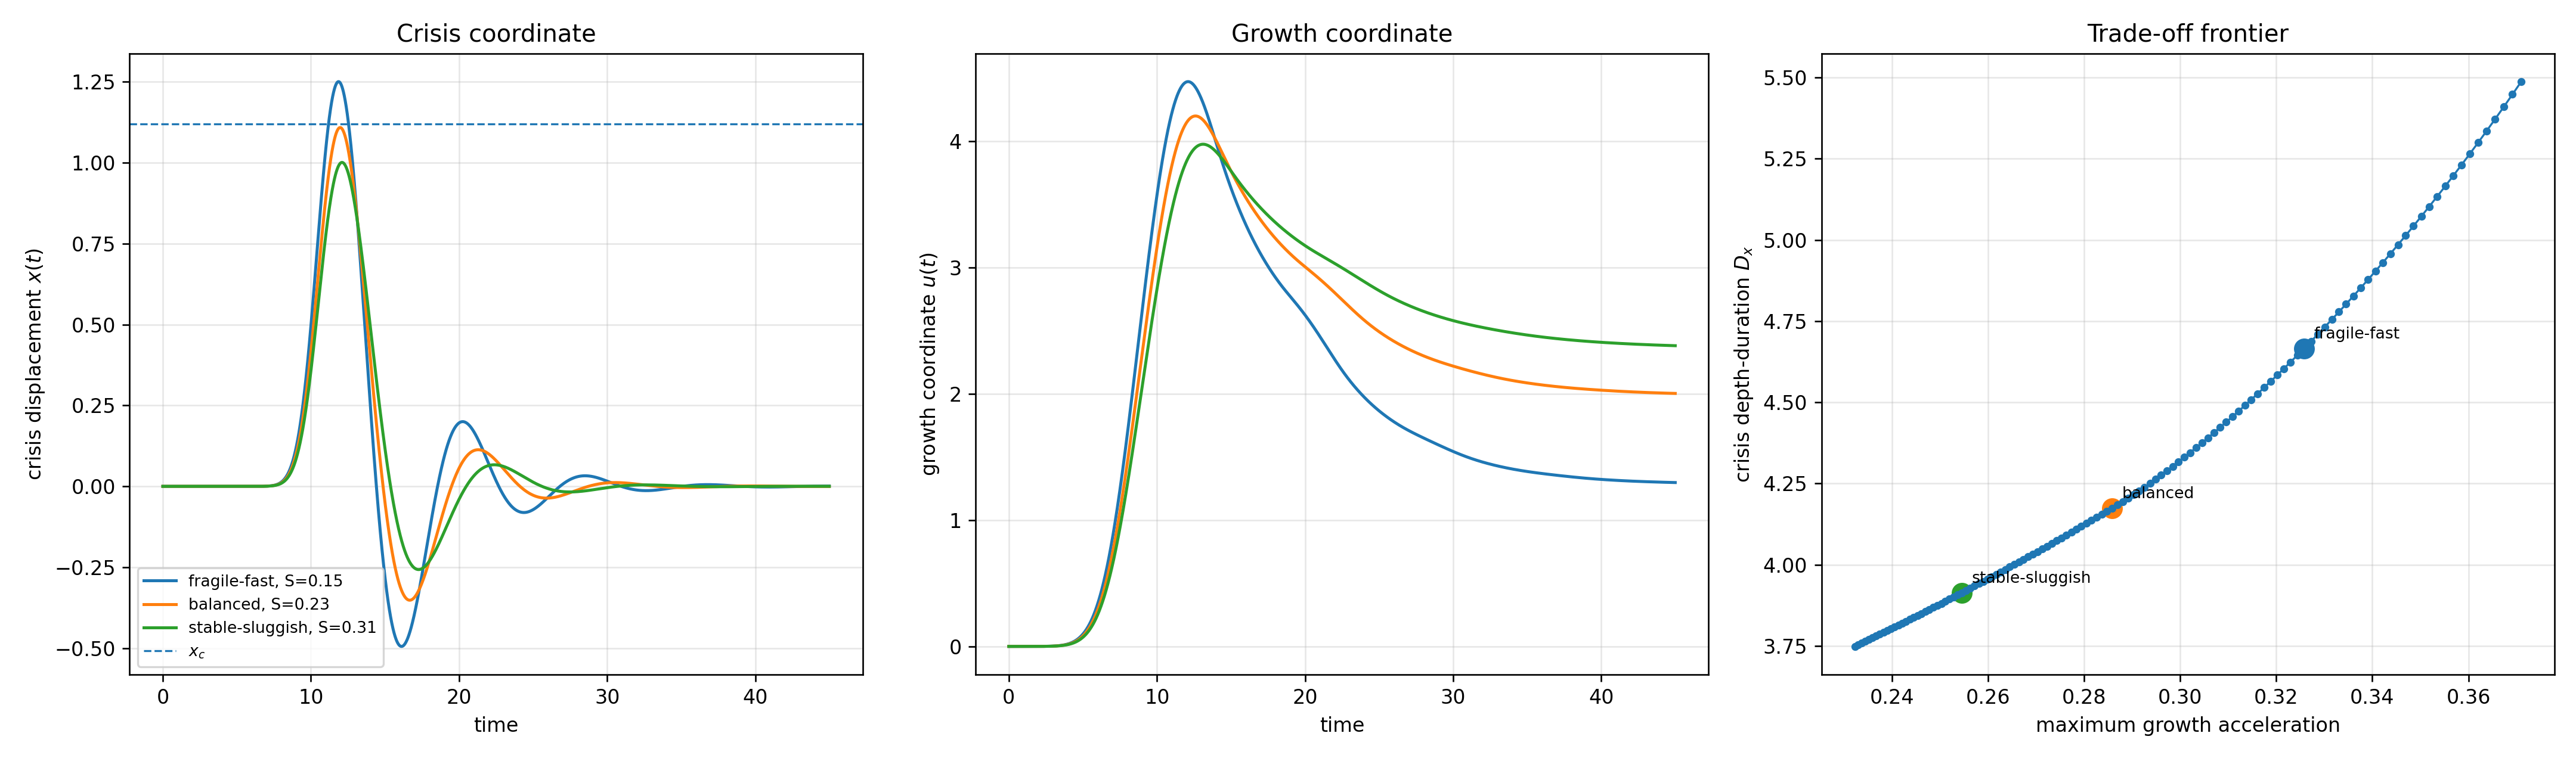
\includegraphics[width=\textwidth]{figures/fig1_toy_trajectories_tradeoff.png}
\caption{Transparent toy oscillator. Low stable inertial mass produces high growth acceleration but crosses the crisis threshold. Intermediate stable mass remains near but below threshold. High stable mass suppresses crisis displacement but reduces growth acceleration. The right panel illustrates the trade-off between crisis depth-duration and maximum tangential growth acceleration across the three regimes.}
\label{fig:toy}
\end{figure}

\begin{figure}[H]
\centering
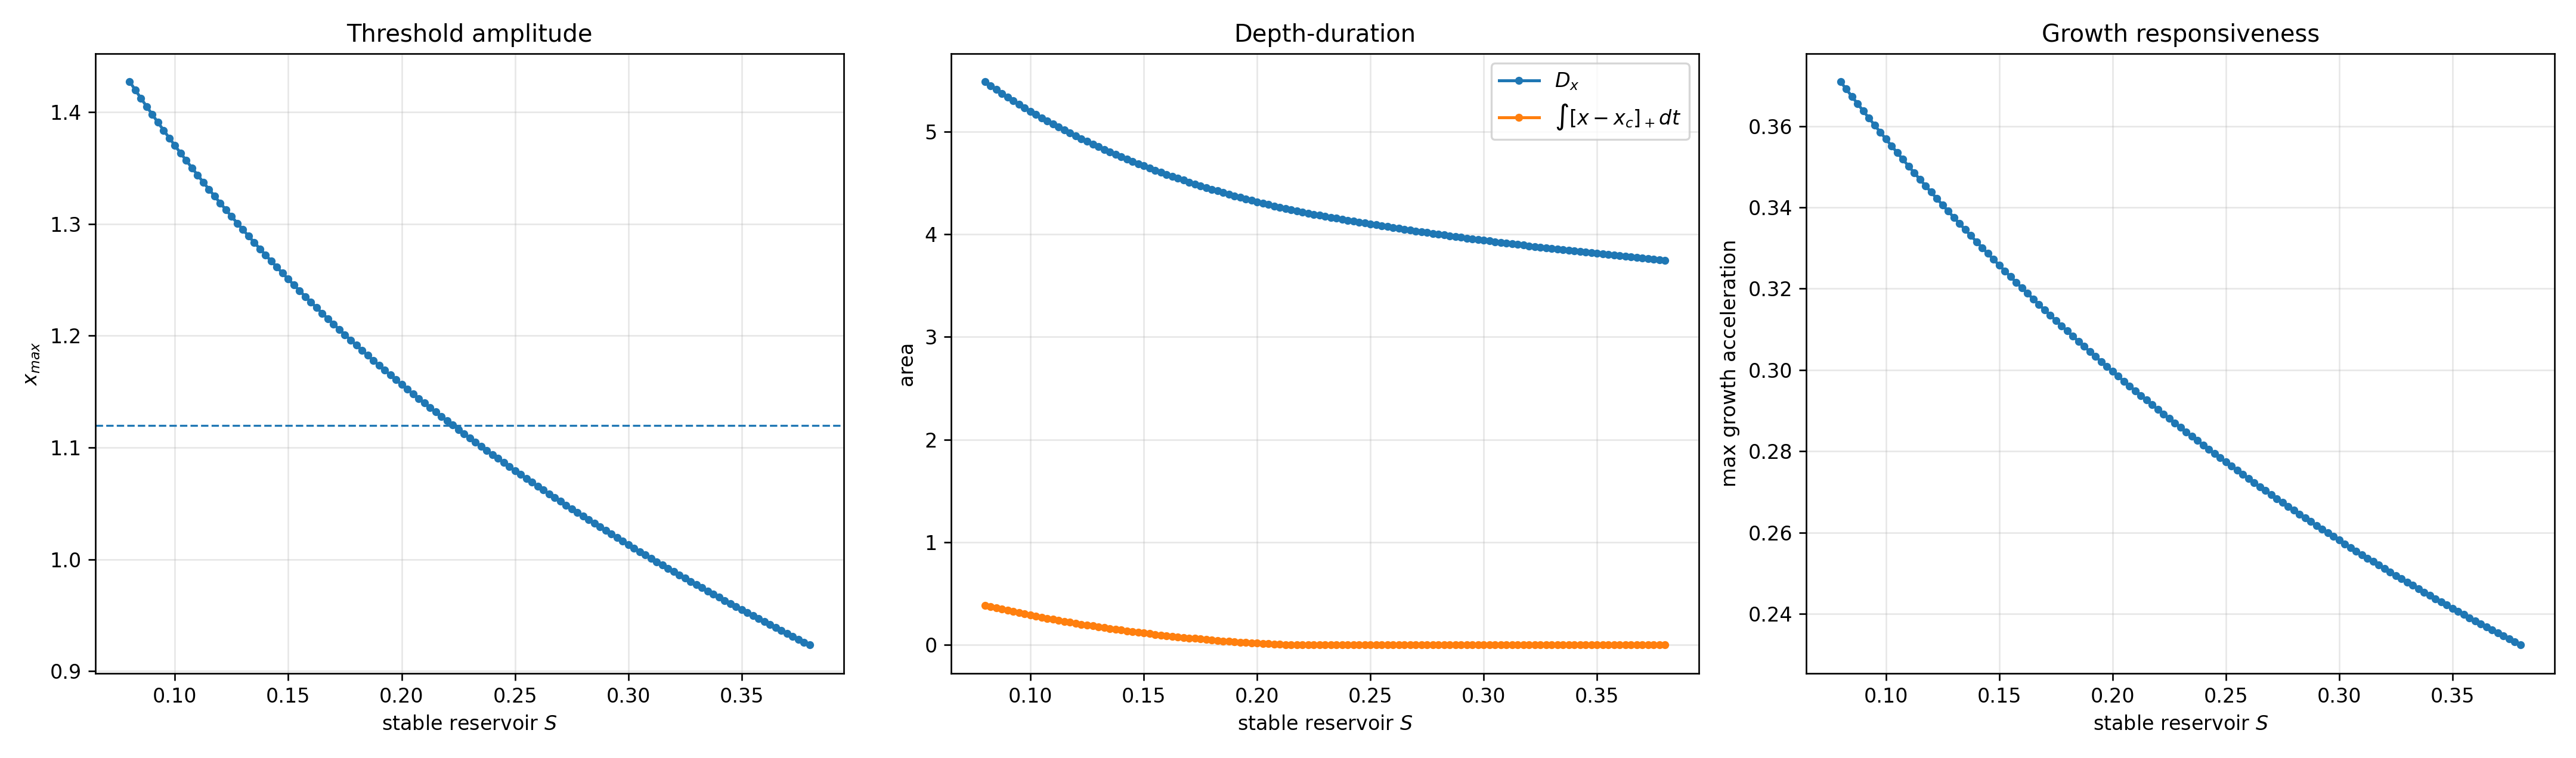
\includegraphics[width=\textwidth]{figures/fig2_stable_mass_scan.png}
\caption{Scanning stable reservoir $S$ in the toy model. Increasing $S$ lowers maximum crisis displacement and accumulated crisis area, but also lowers maximum growth acceleration. This figure illustrates the role of stable inertial mass as both protection and inertia.}
\label{fig:scan}
\end{figure}

The toy regimes are: \emph{fragile-fast} (low $S$, high growth responsiveness, threshold crossing), \emph{balanced} (intermediate $S$, near but below threshold), and \emph{stable-sluggish} (high $S$, crisis suppressed, lower growth acceleration). The labels are conceptual regimes, not fitted empirical clusters.

\subsection{Linear response, damping class, and threshold activation}
\label{sec:linear}
To make the toy trajectories analytically interpretable, the crisis-mode normal form is first examined below threshold. With the threshold term switched off and with no forcing, Eq.~\eqref{eq:crisis} reduces to
\begin{equation}
m(S)\ddot{x}+c_x(S)\dot{x}+k_xx=0.
\label{eq:homogeneous}
\end{equation}
Writing $v=\dot{x}$ gives the equilibrium $(x,v)=(0,0)$ and eigenvalues
\begin{equation}
\lambda_{\pm}(S)=
\frac{-c_x(S)\pm\sqrt{c_x(S)^2-4m(S)k_x}}{2m(S)}.
\label{eq:eigenvalues}
\end{equation}
Thus the unforced subthreshold equilibrium is linearly stable for $m(S)>0$, $c_x(S)>0$, and $k_x>0$. The model time variable is nondimensional; $\omega_x$ is reported in inverse toy-model time units. The natural frequency and damping ratio are
\begin{equation}
\omega_x(S)=\sqrt{\frac{k_x}{m(S)}},
\qquad
\zeta_x(S)=\frac{c_x(S)}{2\sqrt{k_xm(S)}}.
\label{eq:omega_zeta}
\end{equation}
The transition from underdamped to overdamped linear response occurs when
\begin{equation}
c_x(S)^2=4m(S)k_x.
\label{eq:criticaldamping}
\end{equation}
For the parameter values in Table~\ref{tab:toyparams}, Eq.~\eqref{eq:criticaldamping} gives $S\approx -0.237$ and $S\approx 1.848$. The empirical-order range used in the toy simulation, $S=0.15$--$0.31$, therefore lies in the underdamped regime, with $\zeta_x\approx0.28$--$0.39$. For all physically meaningful stable-reservoir values in the illustrative range, the model remains underdamped. Stable inertial mass does not remove oscillatory response in this range; rather, it reduces the amplitude and moves the system relative to the crisis threshold. The linearization, damping classification, and phase-plane representation follow standard nonlinear-oscillation and dynamical-systems practice \cite{GuckenheimerHolmes1983}.

\begin{figure}[H]
\centering
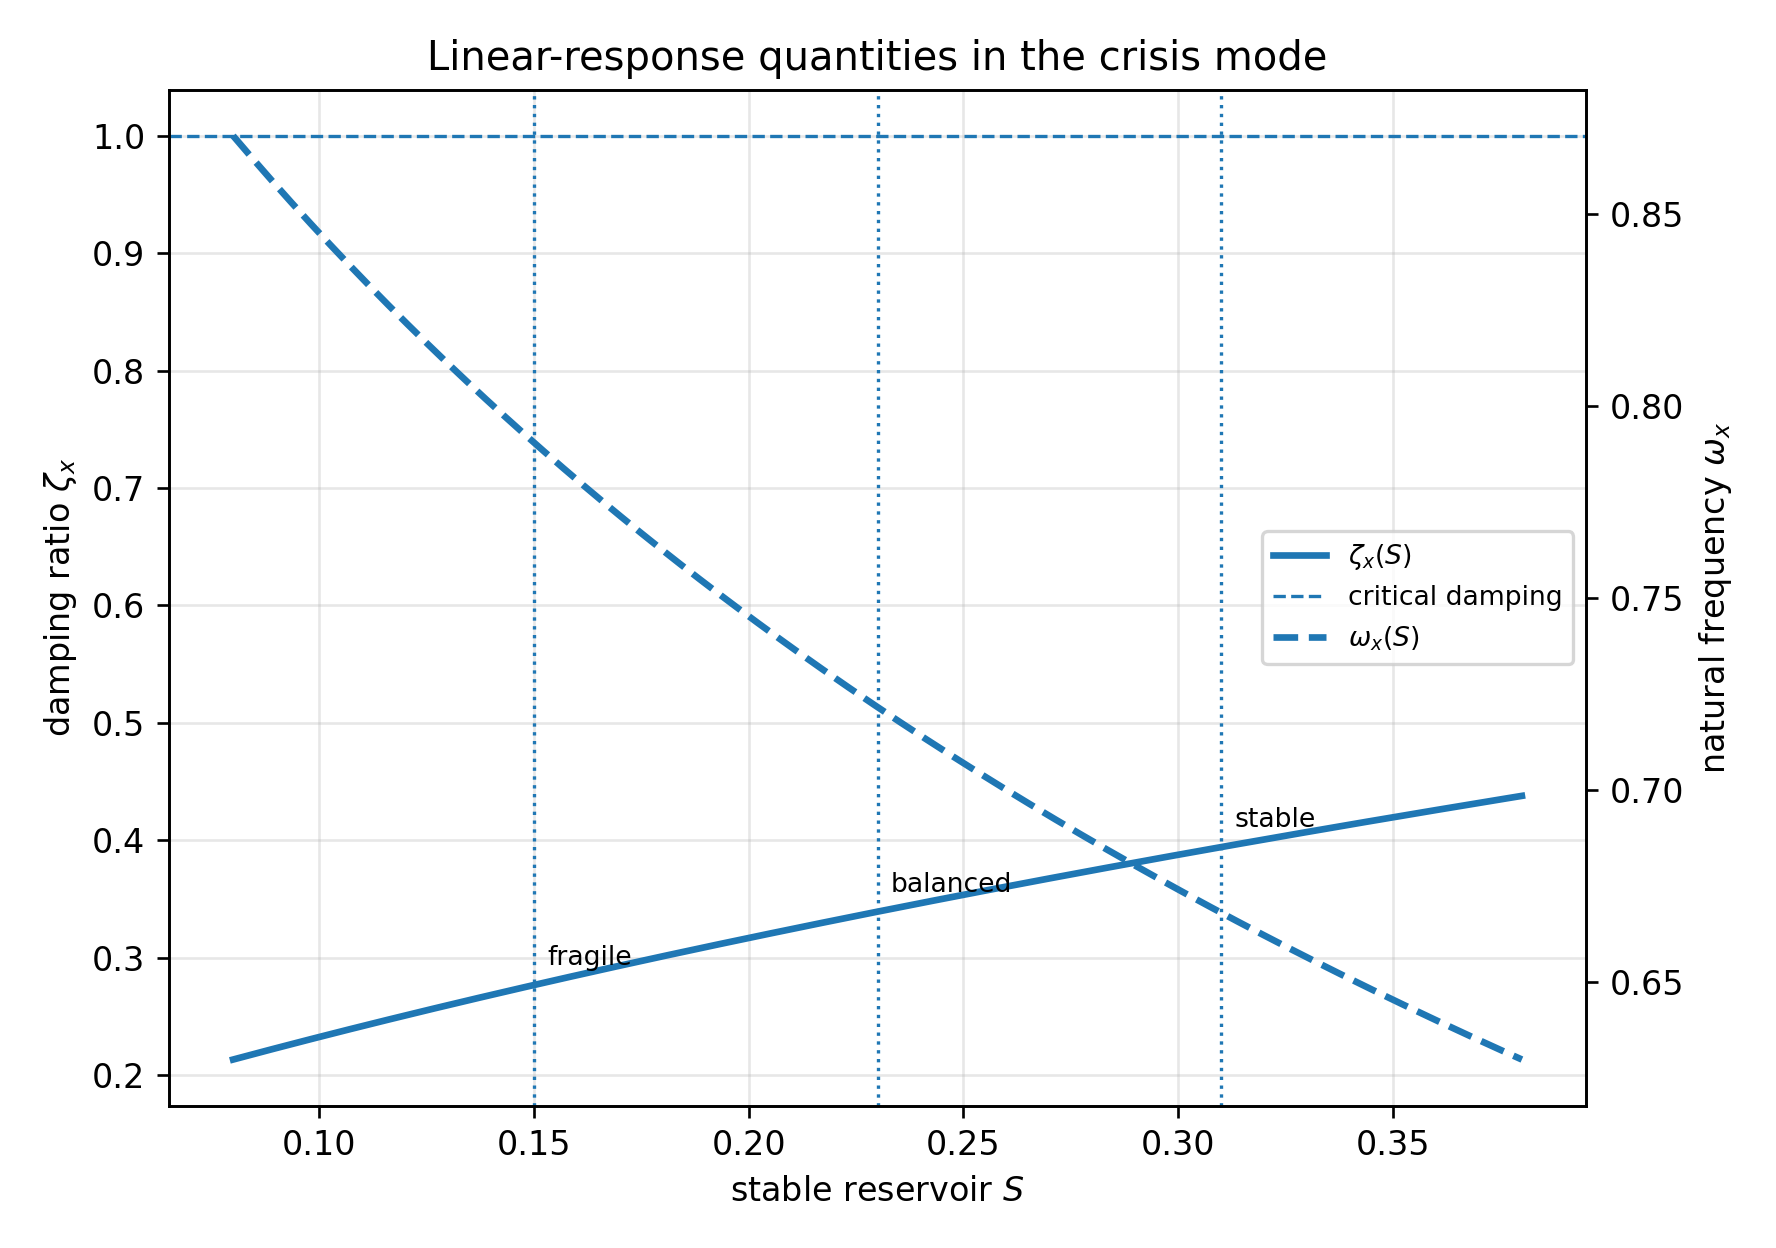
\includegraphics[width=0.82\textwidth]{figures/fig3_linear_response_functions.png}
\caption{Linear-response quantities in the crisis mode. The stable reservoir $S$ increases the damping ratio $\zeta_x(S)$ and decreases the natural frequency $\omega_x(S)$ over the illustrative range. The natural frequency is reported in inverse nondimensional toy-model time units. The toy regimes remain underdamped in this range, so the role of $S$ is not to eliminate oscillatory response but to reduce the forced displacement relative to the threshold $x_c$.}
\label{fig:linearresponse}
\end{figure}

For the Gaussian crisis pulse defined above, the forcing amplitude enters through
\begin{equation}
F_x(t)=A_x f_x(t).
\end{equation}
Let $x_{\mathrm{lin}}(t;S,A_x)$ be the solution of the linear subthreshold problem. A useful threshold-control number is
\begin{equation}
\mathcal{C}(S,A_x)=
\frac{\max_t x_{\mathrm{lin}}(t;S,A_x)}{x_c}.
\label{eq:Cthreshold}
\end{equation}
If $\mathcal{C}<1$, the pulse remains an ordinary fluctuation in the linear subthreshold regime. If $\mathcal{C}>1$, the system crosses the crisis threshold and activates the nonlinear term $\kappa\brpos{x-x_c}$. Because $x_{\mathrm{lin}}$ is proportional to $A_x$ in the subthreshold problem, the threshold boundary in the $(S,A_x)$ plane is equivalently given by $\mathcal{C}(S,A_x)=1$. Thus $S_{\mathrm{crit}}$ is not a universal number; it is the critical reservoir value for a specified pulse amplitude and width. For the baseline toy forcing amplitude $A_x=1.22$, the linear threshold condition gives
\begin{equation}
S_{\mathrm{crit}}\approx0.223,
\qquad
\max_t x_{\mathrm{lin}}(t;S_{\mathrm{crit}},A_x)=x_c.
\label{eq:Scrit}
\end{equation}
Thus the illustrative regimes straddle the threshold: $S=0.15$ crosses, $S=0.23$ sits near the transition, and $S=0.31$ remains below threshold. This is the dynamical basis of the fragile-fast, balanced, and stable-sluggish labels.

\begin{figure}[H]
\centering
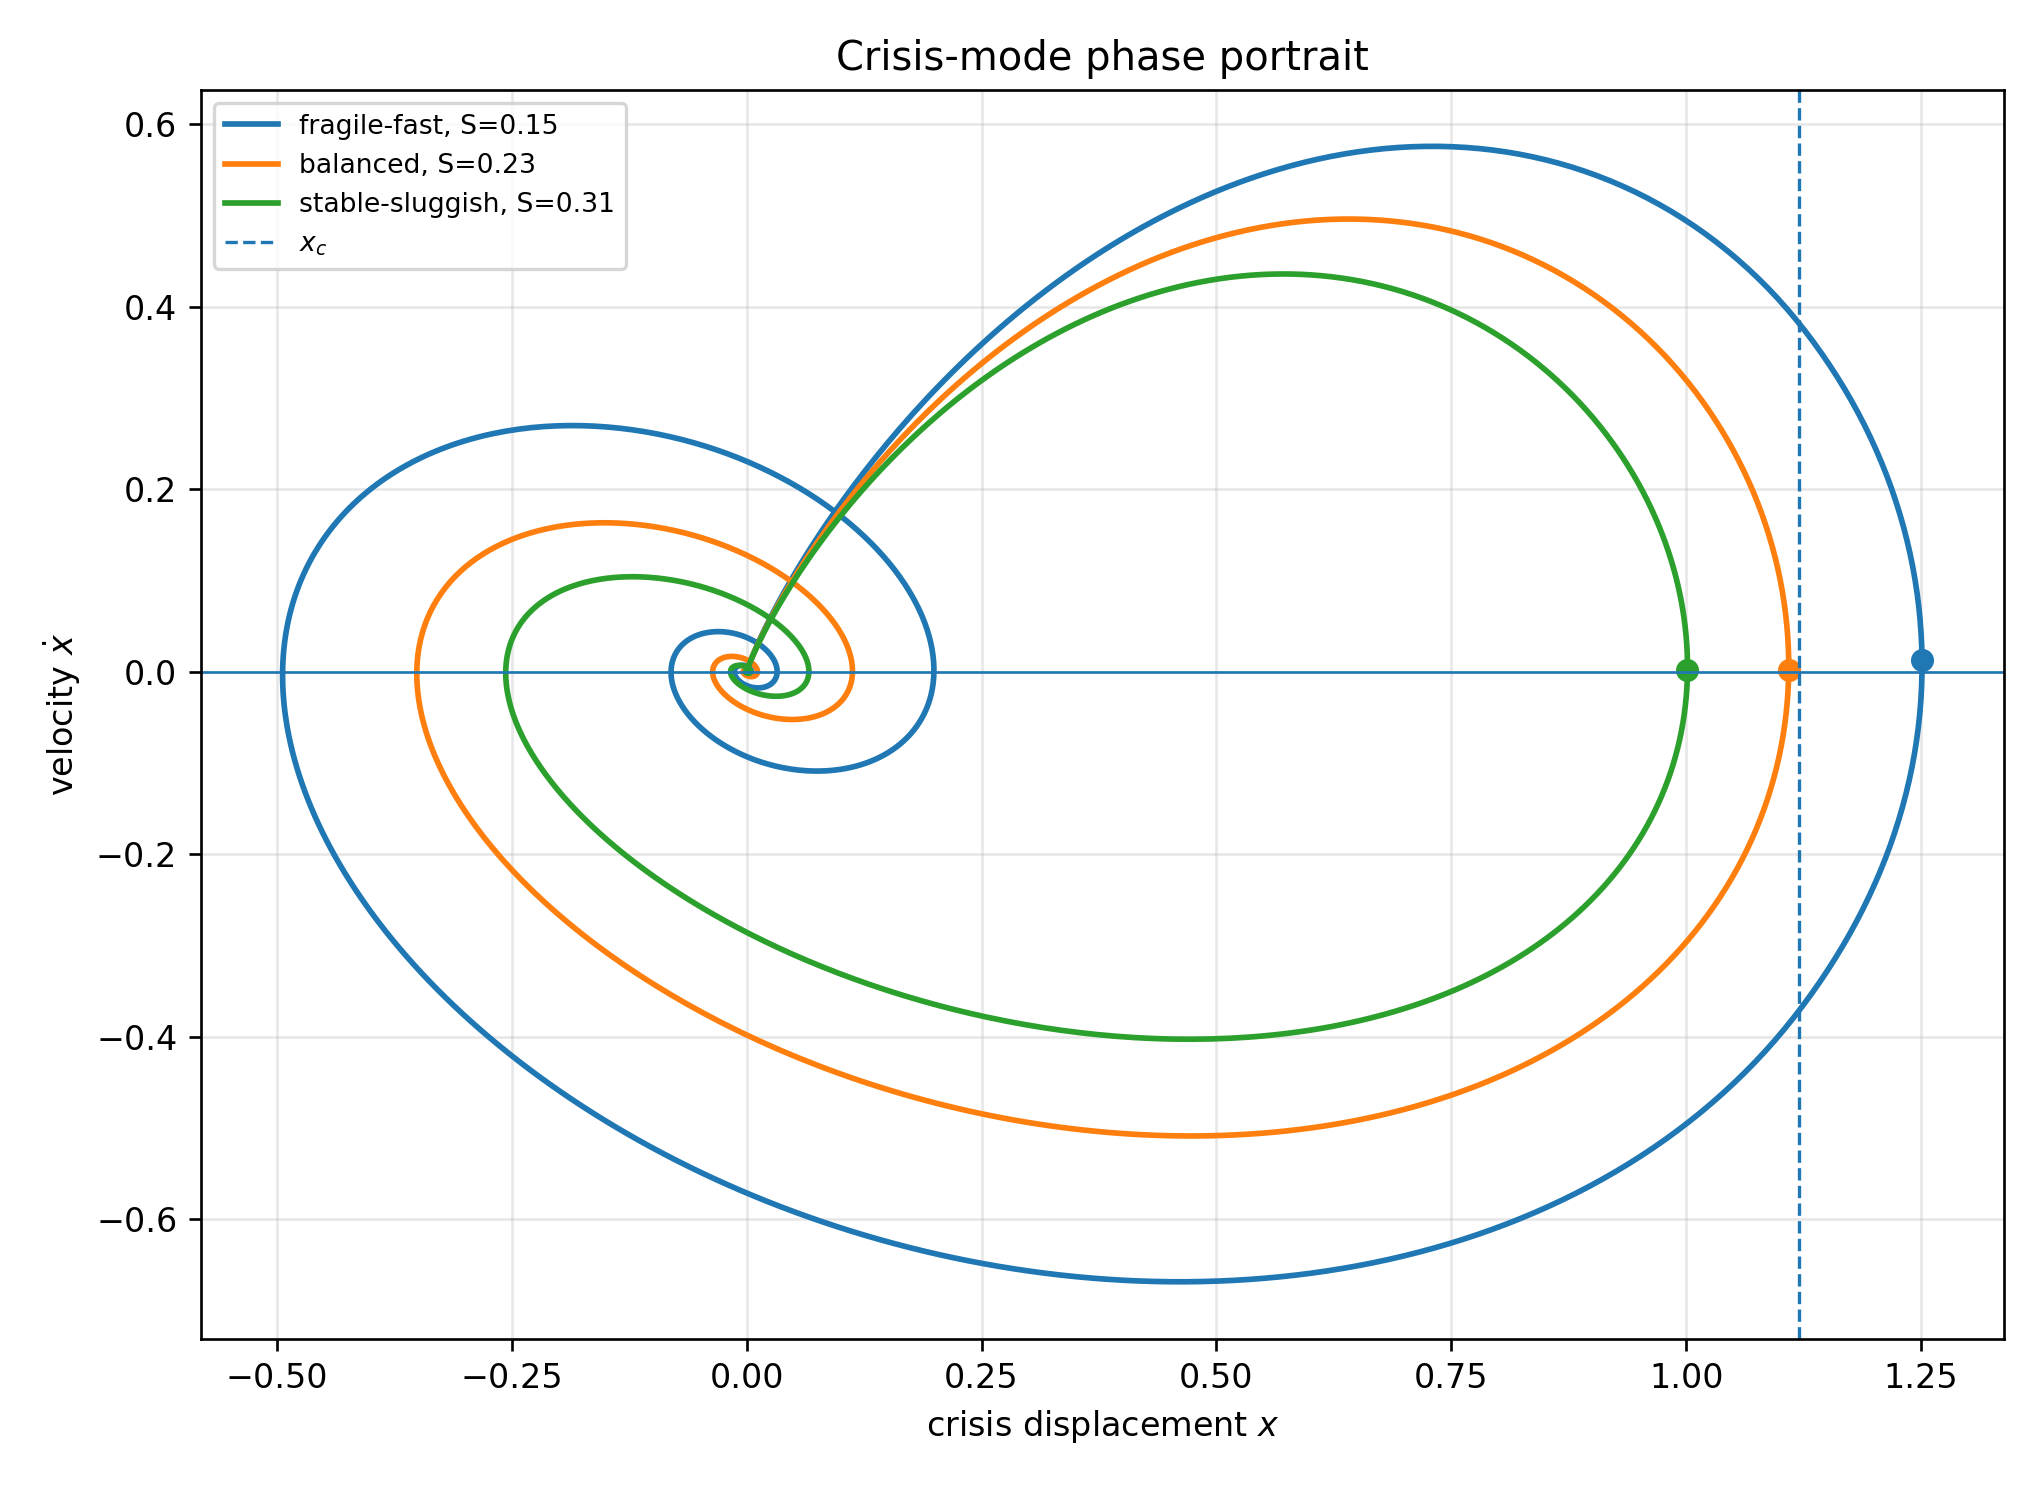
\includegraphics[width=0.92\textwidth]{figures/fig4_phase_portrait.png}
\caption{Crisis-mode phase portrait in the $(x,\dot{x})$ plane for the three toy regimes. The vertical dashed line marks the crisis threshold $x_c$. The low-$S$ trajectory crosses the threshold, the intermediate case lies close to it, and the high-$S$ trajectory remains below it. The figure shows that the regime labels refer to motion in phase space, not only to time-series amplitudes. The point of comparison is not a change in attractor structure but a change in excursion scale: the trajectories retain the same finite-pulse response geometry while stable inertial mass contracts the phase-space loop relative to $x_c$. The response is finite-pulse and does not include a second attractor.}
\label{fig:phaseportrait}
\end{figure}

The present paper studies threshold-amplified transients, not persistent crisis basins. Above the threshold, the nonlinear term $\kappa\brpos{x-x_c}$ amplifies the transient displacement but does not create a second attractor in the present minimal model. Since the forcing is a finite pulse and the baseline system remains damped and restoring, trajectories eventually decay back toward the origin. Persistent crisis states would require an additional damage variable, state-dependent stiffness, sustained forcing, or a second basin of attraction; these extensions are left for future work. For weak threshold activation, the leading above-threshold burden can be read as a residence-time correction around the subthreshold response. The approximation is intended for the regime in which the nonlinear impulse above threshold remains small relative to the linear damping scale, for example $\kappa\max_t\brpos{x_{\rm lin}(t)-x_c}\ll c_x(S)\omega_x$, where $x_{\rm lin}$ is the corresponding subthreshold linear response and $\omega_x=\sqrt{k_x/m(S)}$. In this regime,
\begin{equation}
D_x \approx \int \brpos{x_{\mathrm{lin}}(t;S,A_x)-x_c}\,dt,
\label{eq:dxresidence}
\end{equation}
with nonlinear amplification increasing with both the excess amplitude above $x_c$ and the time spent above the boundary. This approximation explains why the threshold-regime map is organized primarily by the contour $\mathcal{C}(S,A_x)=1$ rather than by a change in attractor topology.

\begin{figure}[H]
\centering
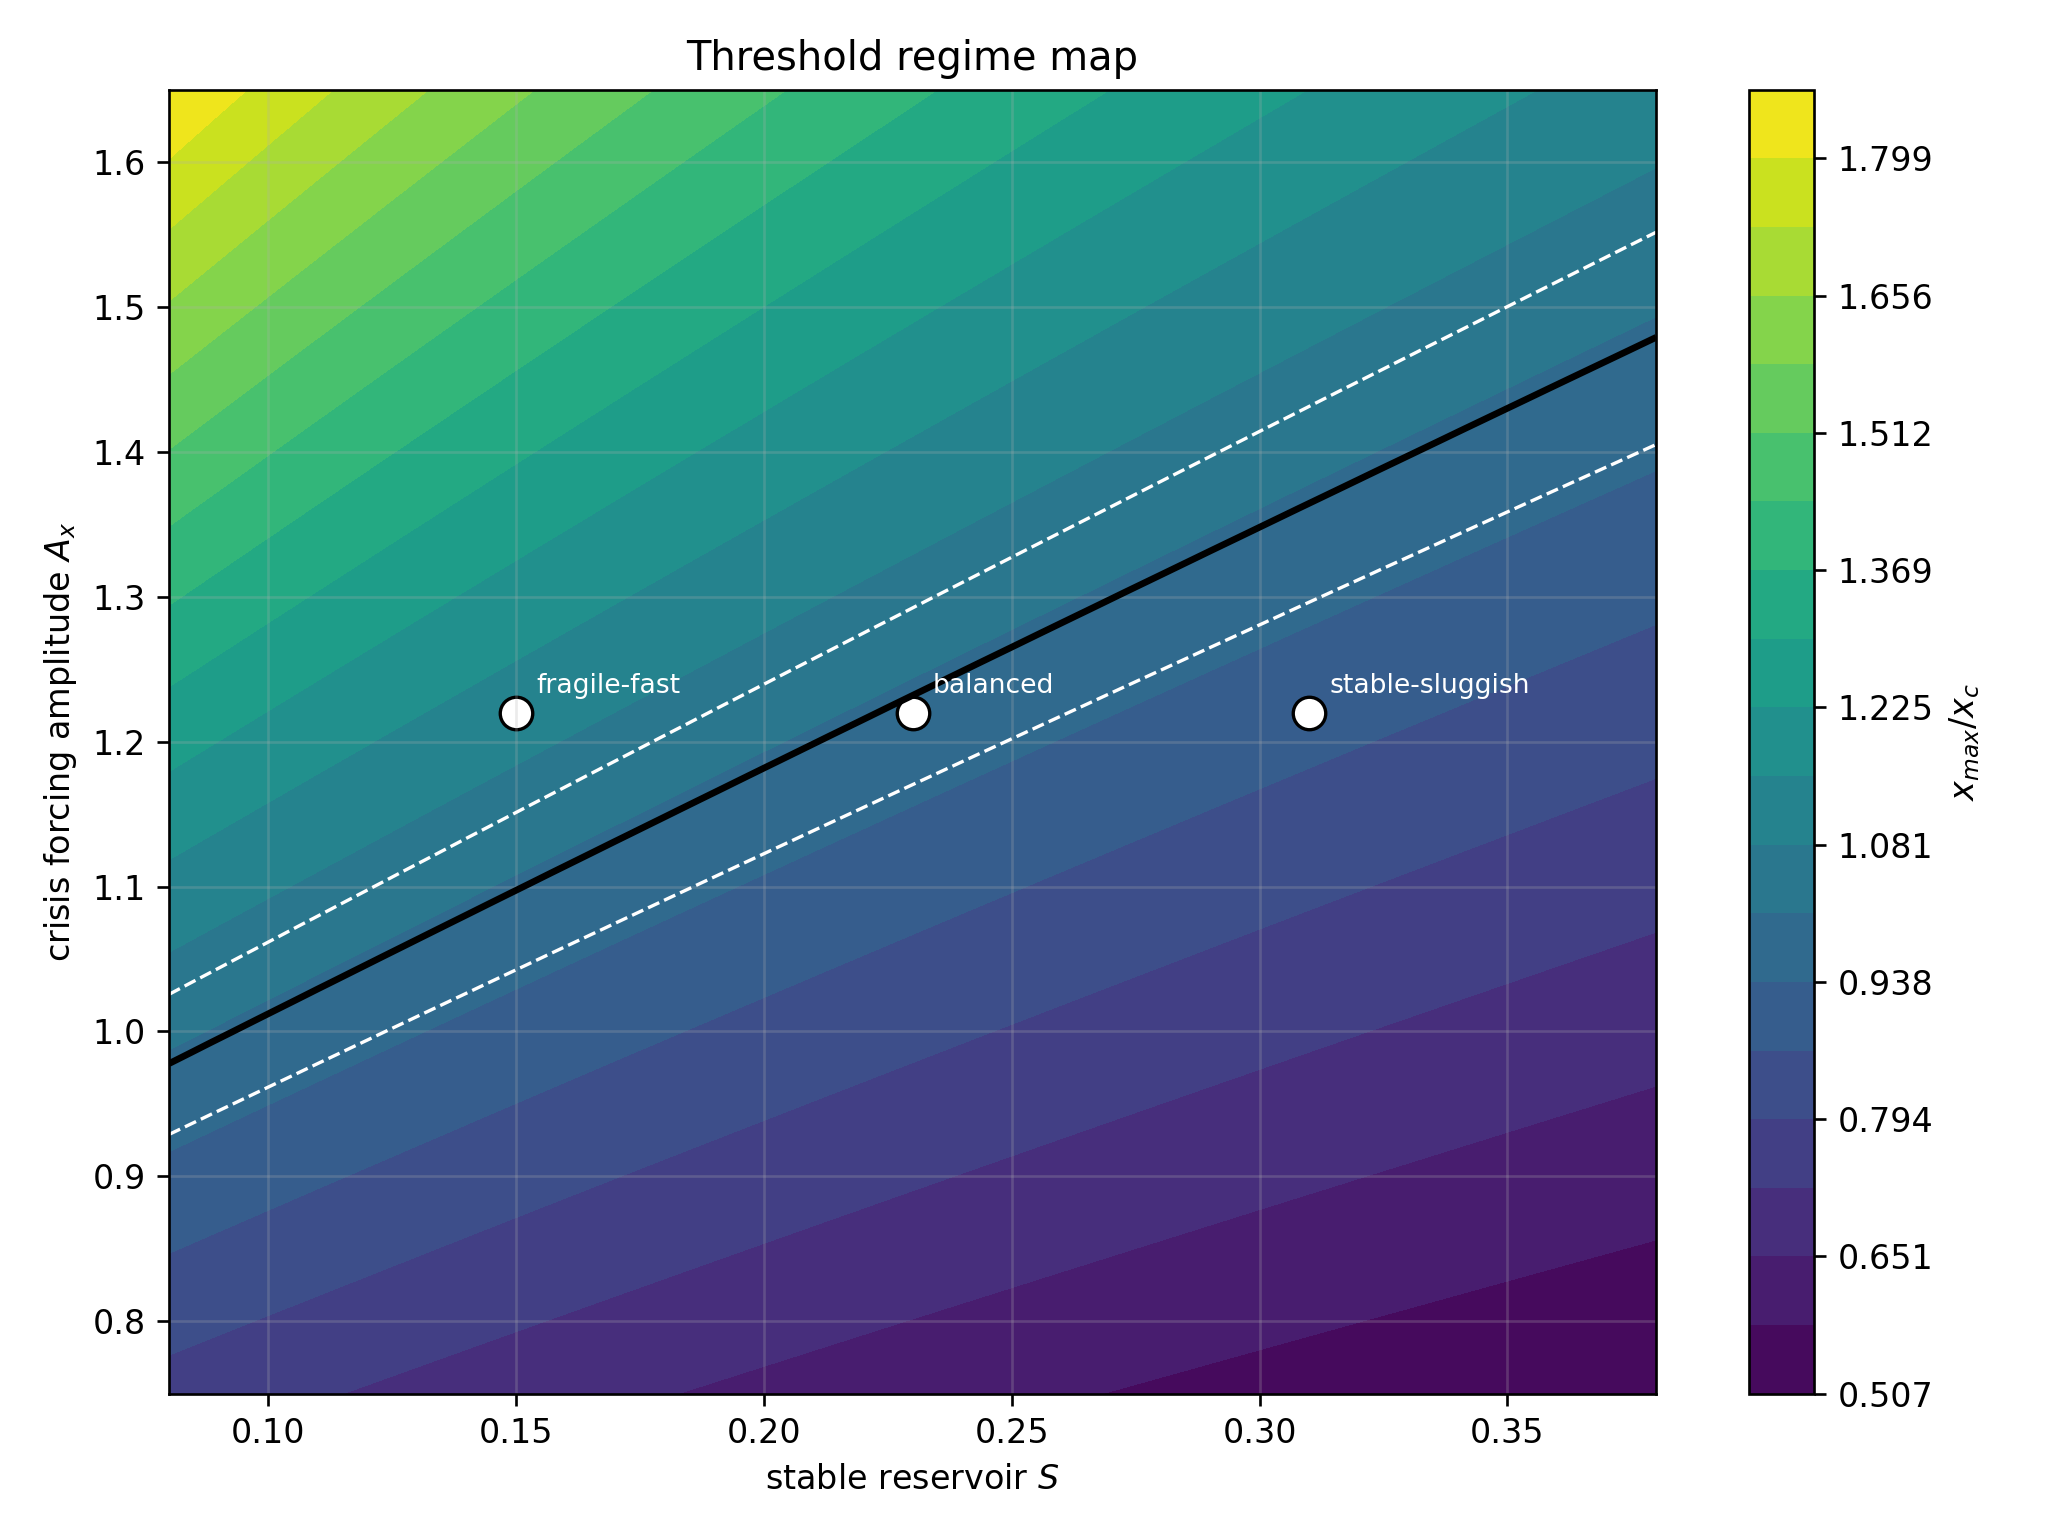
\includegraphics[width=0.92\textwidth]{figures/fig5_threshold_regime_map.png}
\caption{Threshold regime map for the toy crisis mode in the $(S,A_x)$ plane. Color shows $x_{\max}/x_c$ computed from the transparent toy model with the threshold feedback active. The solid black contour marks the threshold condition $x_{\max}=x_c$; dashed contours mark a narrow transition band around it. The three white points are the toy regimes used in Fig.~\ref{fig:toy}. The vertical axis is the abstract crisis-forcing amplitude $A_x$; the empirical exposure proxy $E_H=X+I+\brpos{H-H_c}$ is introduced later as one possible mapping onto this amplitude, not as part of the basic normal form. The near-linearity of the boundary reflects the slow variation of the subthreshold gain $G(S)$ over the illustrative $S$ range.}
\label{fig:thresholdmap}
\end{figure}


\subsection{Empirical scaling and country archetypes}
\label{sec:empirical}
The narrow empirical proxy remains Eq.~\eqref{eq:Z1}. It is a coarse empirical projection of the dynamical ratio $S/F_x$: $\Sigma$ approximates a measured component of the stable reservoir, while $E_H=X+I+\brpos{H-H_c}$ approximates transverse forcing amplitude. The country mapping is archetypal rather than a fitted classification.

The processed empirical variables are drawn from OECD SOCX for public social expenditure, BIS total-credit statistics for household credit, and World Bank WDI for GDP, household consumption, exports, investment, and population series \cite{OECD_SOCX,BIS_TC,WorldBank_WDI}. The empirical layer uses two explicitly separated samples. The \emph{core sample} contains countries with complete inputs for the $Z_1$ scaling: $\Sigma$, $X$, $I$, $H$, $R_{2009}$, $D_C$, and growth-side diagnostics. The \emph{extended WDI diagnostic sample} contains countries for which the WDI time-series quantities needed for $D_C$ and $\Delta F_u$ are available, even if the stabilizer or household-debt inputs required for $Z_1$ are incomplete in the processed pilot table. Extended-sample countries are not used to support the $Z_1$ scaling claim. The construction of the consumption depth-duration coordinate is given explicitly in Materials and Methods.

\begin{table}[H]
\centering
\caption{Data-layer definition used in the pilot. The separation prevents countries with incomplete stabilizer/exposure inputs from being mixed into the $Z_1$-based scaling panels.}
\label{tab:coverage}
\begin{tabular}{p{0.22\textwidth}p{0.36\textwidth}p{0.28\textwidth}}
\toprule
Layer & Required quantities & Countries used \\
\midrule
Core $Z_1$ scaling sample & $\Sigma,X,I,H,Z_1,R_{2009},D_C,F_u$ diagnostics & CAN, DEU, DNK, ESP, FIN, FRA, GBR, IRL, ITA, JPN, NLD, SWE, USA \\
Extended WDI diagnostic sample & $D_C,F_u^{post},\Delta F_u$ from WDI time series & Core sample plus AUT, BEL, CHE \\
Reference point & Static stabilizer/exposure values; not part of crisis-country regression & ISR \\
\bottomrule
\end{tabular}
\end{table}

\begin{figure}[H]
\centering
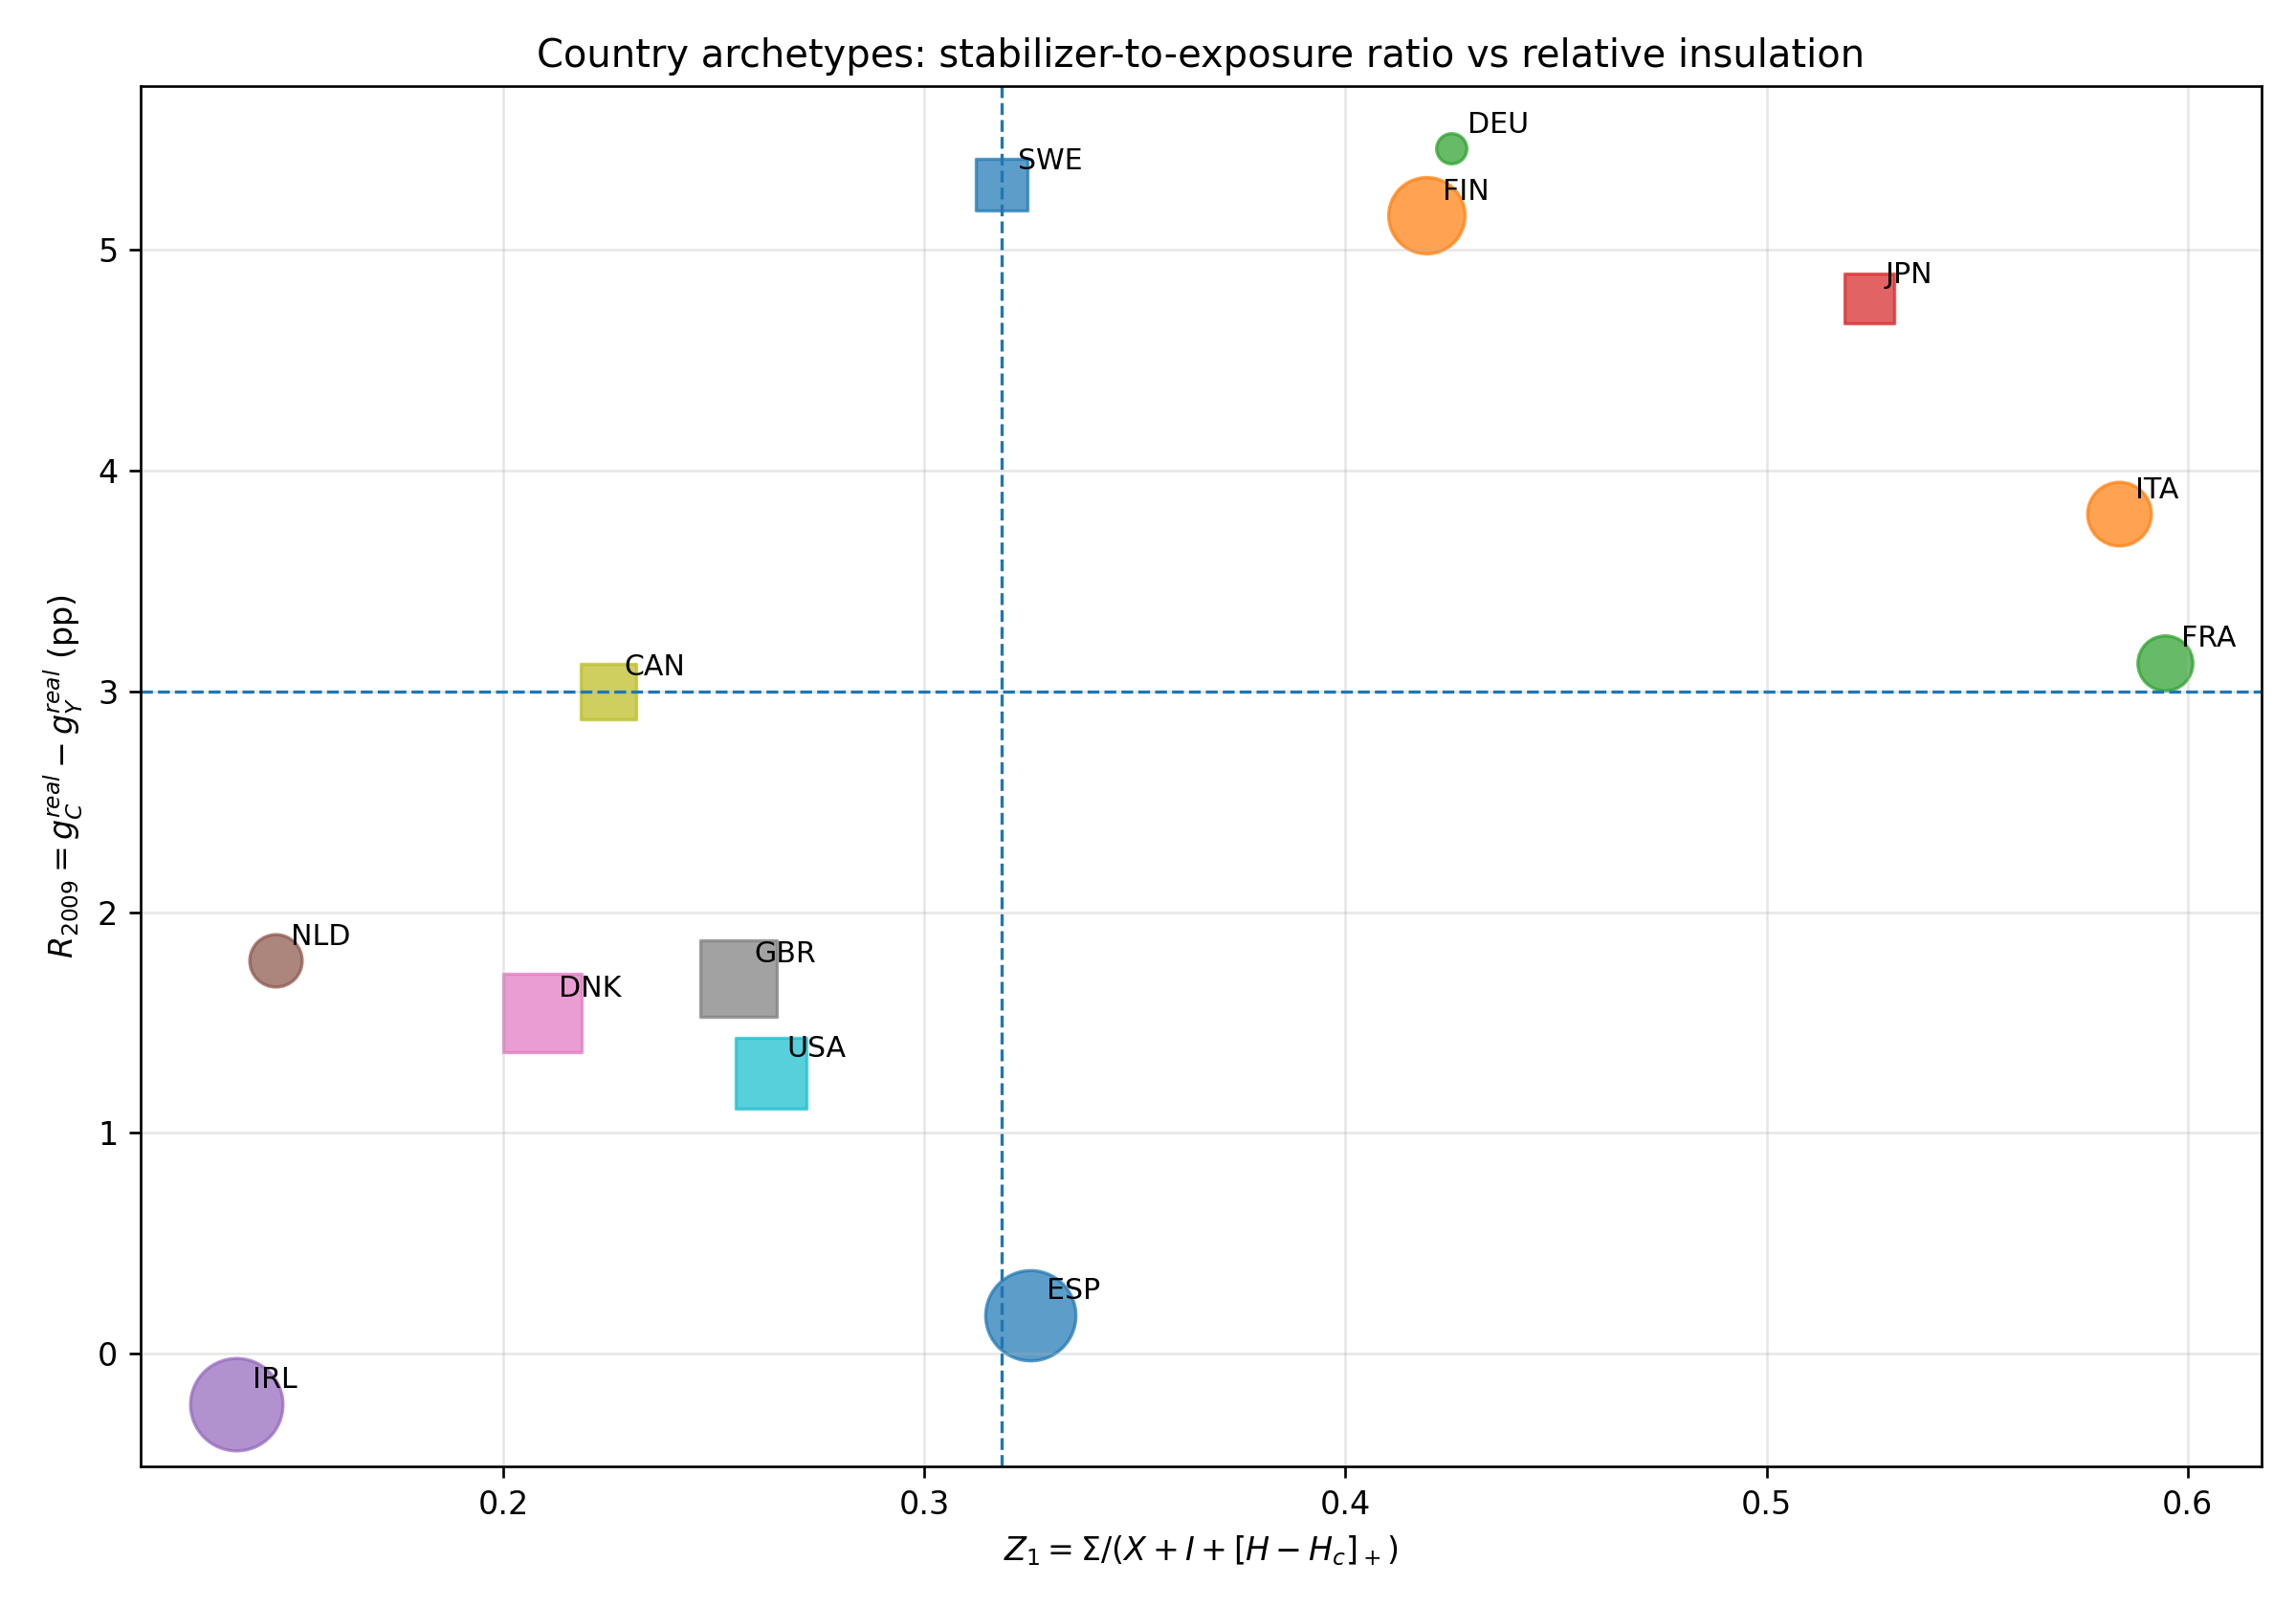
\includegraphics[width=0.95\textwidth]{figures/fig6_country_archetypes_Z1_R.png}
\caption{Country archetypes in the plane of stabilizer-to-exposure ratio $Z_1$ and shock-year relative insulation $\Rbuffer=g^{real}_{C,2009}-g^{real}_{Y,2009}$. Marker size indicates consumption depth-duration. Israel is shown only as a non-recession reference point: its household-debt ratio is below the baseline threshold $H_c$, so the thresholded balance-sheet fragility channel is inactive and the point is not included in the recession-country regression.}
\label{fig:countryR}
\end{figure}

\begin{figure}[H]
\centering
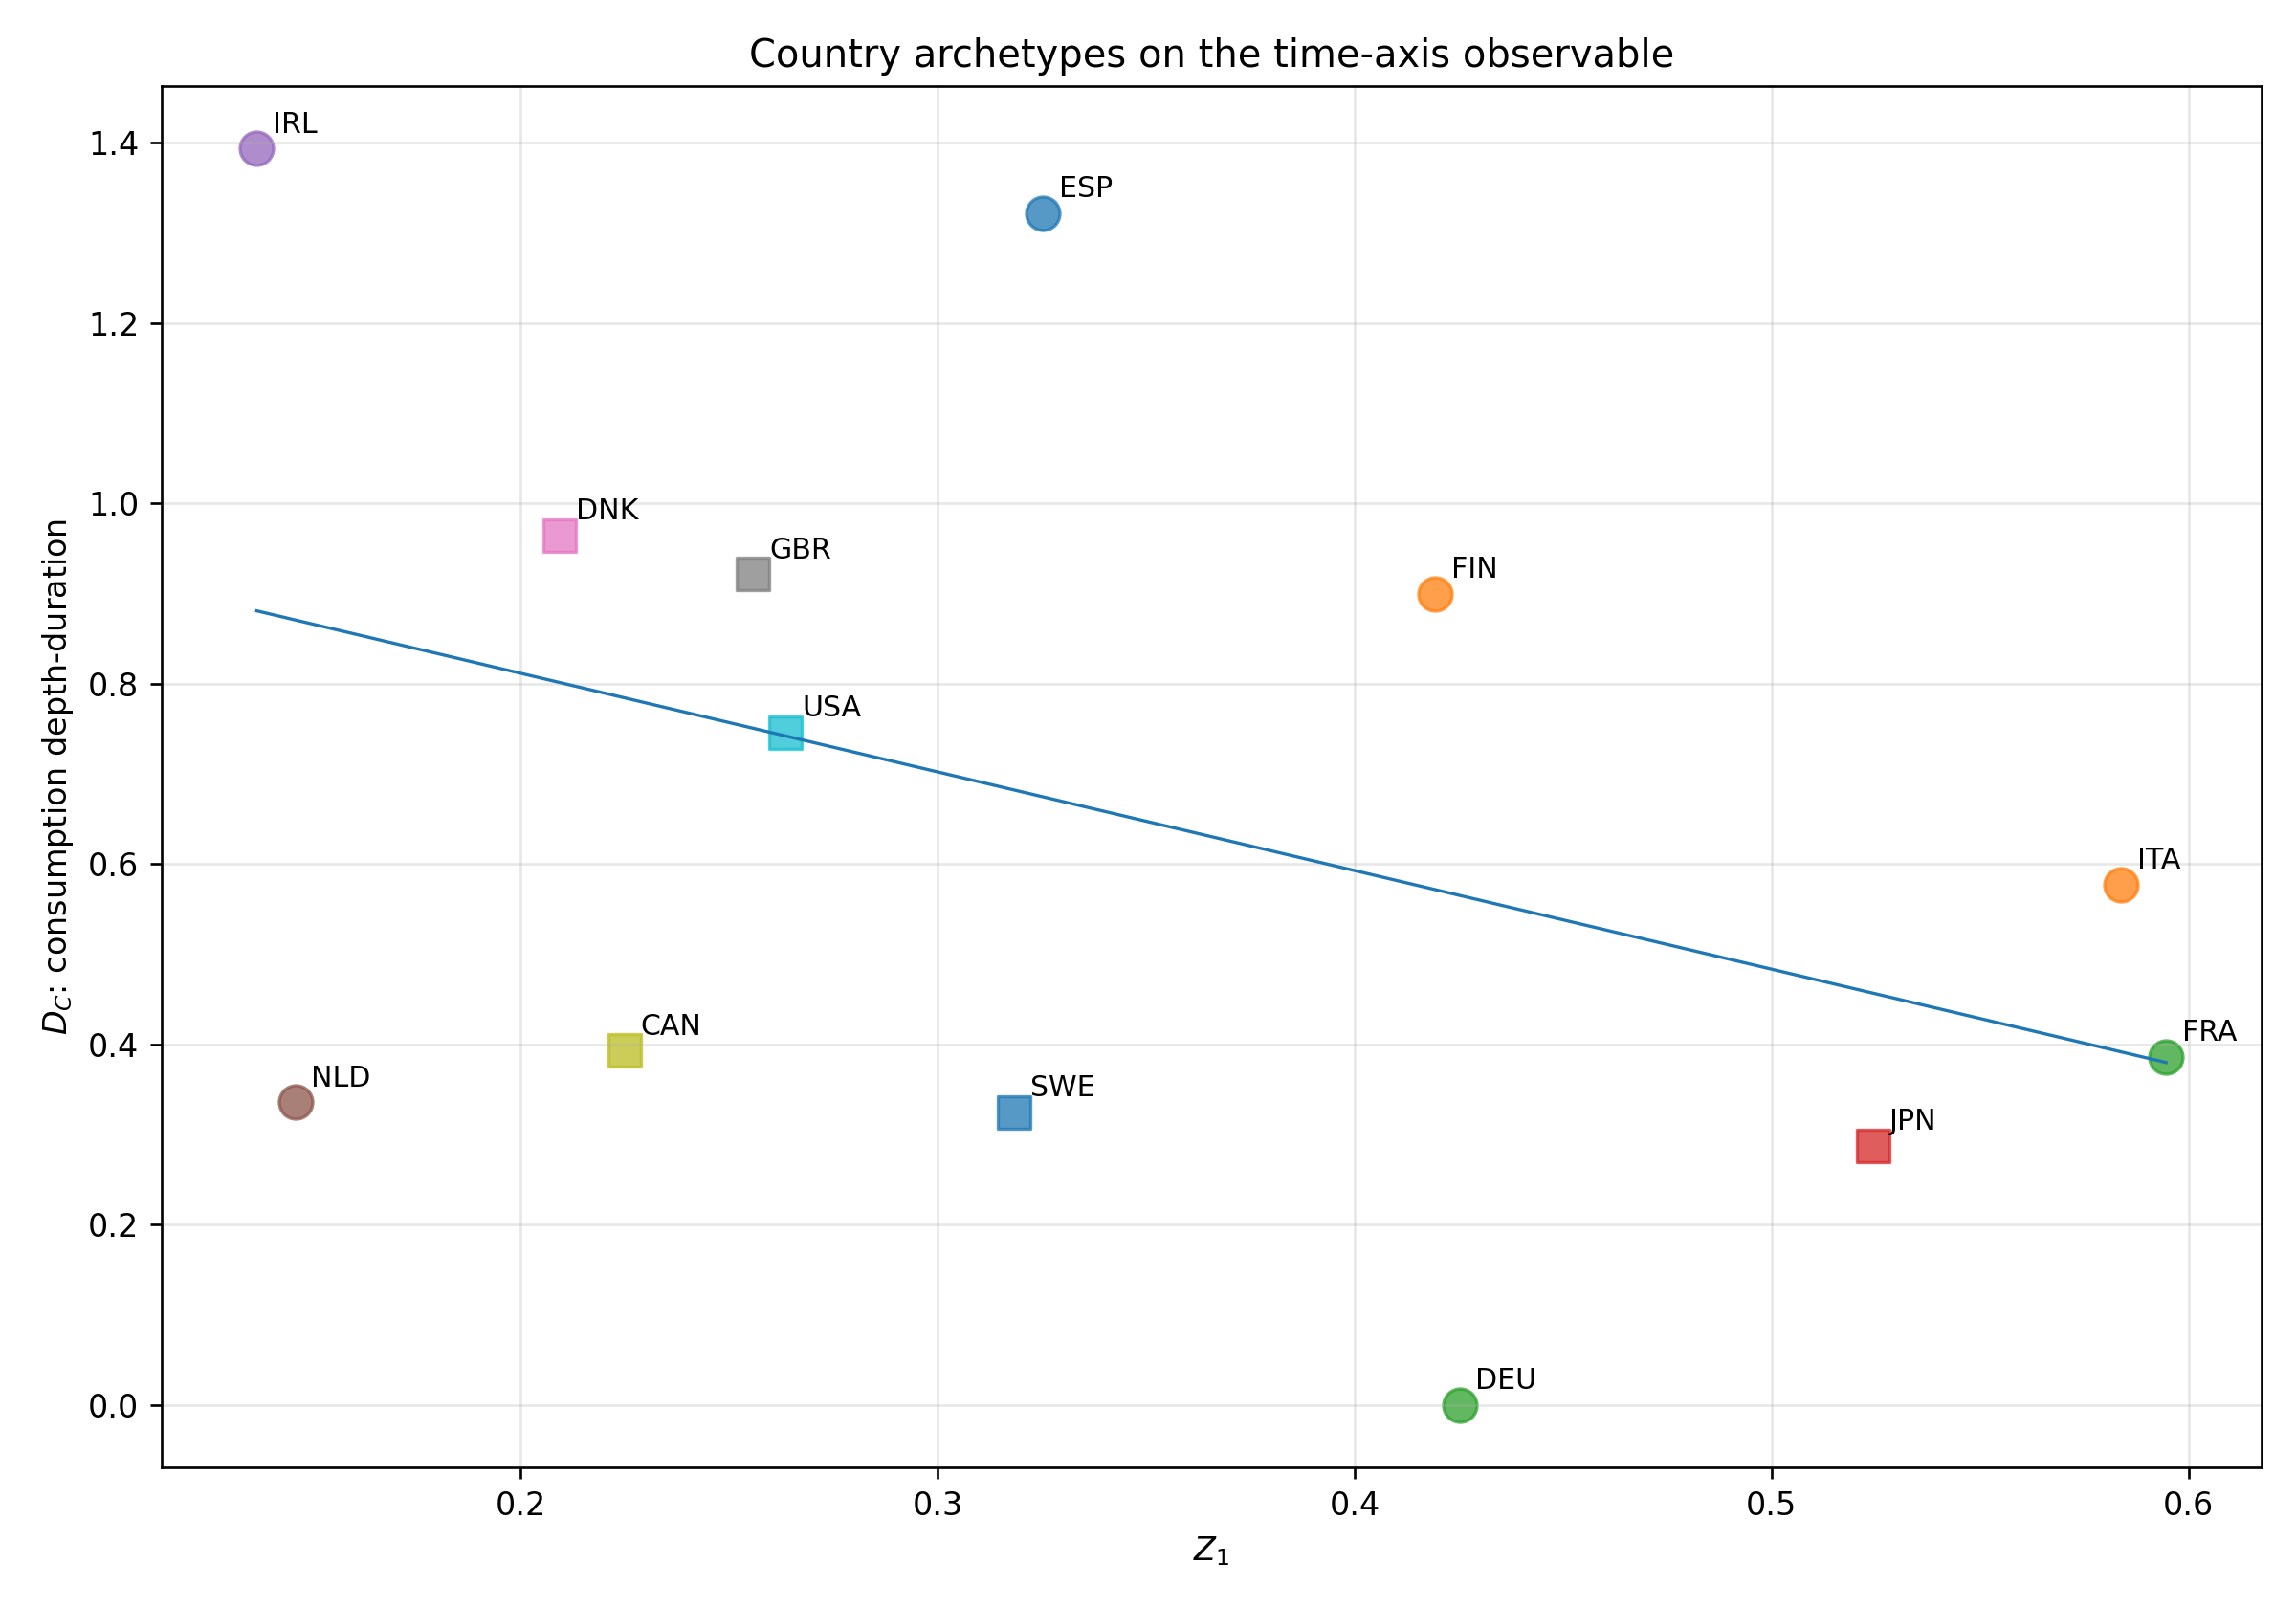
\includegraphics[width=0.95\textwidth]{figures/fig7_country_archetypes_Z1_DC.png}
\caption{Country archetypes on the time-axis observable $D_C$. The direction is consistent with the interpretation of $Z_1$ as a shock-absorption parameter, but the sample is small and the figure should be read as diagnostic.}
\label{fig:countryDC}
\end{figure}

Germany, Sweden, Finland, and Japan appear as balanced/buffered cases. Ireland, the Netherlands, Denmark, and the United Kingdom illustrate debt-fragile leveraged cases: stable reservoirs may exist, but household leverage raises transverse exposure. Spain, the United States, and Canada are threshold-prone or fragile-fast candidates, with Canada more ambiguous. France and Italy are stable-sluggish candidates, but the sluggish part of the label requires a growth-axis observable. Israel is best read as a threshold-avoidance reference: household debt was below the fragility threshold, so the balance-sheet fragility channel was not activated.

Austria, Belgium, and Switzerland appear only in the extended WDI growth-side diagnostics because the required WDI time series are available. They are not used in the main $Z_1$ scaling interpretation because stabilizer or household-debt inputs are incomplete in the processed pilot table. For the present pilot, these countries remain restricted to the extended diagnostic panels.

\subsection{Post-crisis growth forcing and the coupling term}
The immediate rebound proxy
\[
A_g=g_{Y,2010}-g_{Y,2009}
\]
is not a pure growth-forcing observable. It mixes intrinsic responsiveness with rebound from damage. We therefore define a cruder post-rebound growth-slope proxy,
\[
F_u^{post}=\overline{g}_{Y,2011-2013},
\]
and a change relative to the pre-crisis growth slope,
\[
\Delta F_u=\overline{g}_{Y,2011-2013}-\overline{g}_{Y,2004-2007}.
\]
These quantities are not measurements of the ODE forcing term; they are transparent empirical proxies for the post-rebound tangential growth environment.

The strongest diagnostic signal in the growth-side pilot is not between $\Sigma$ and post-growth slope, but between crisis depth-duration and deterioration in post-crisis growth slope. Across the current extended WDI diagnostic sample ($n=16$), $D_C$ and $\Delta F_u$ are correlated at
\[
r=-0.63,
\qquad 95\%\ \mathrm{CI}\approx[-0.86,-0.19],
\]
using a Fisher-$z$ interval. This is consistent with the coupling term $-\lambda x_+(t)$ in Eq.~\eqref{eq:growth}: persistent transverse displacement is associated with weaker subsequent tangential growth. It is not a causal identification. Weak post-crisis growth capacity may also contribute to persistent consumption gaps. The present pilot therefore treats the relation as a diagnostic consistency check, not as an estimate of $\lambda$.

Figure~\ref{fig:FuPhase} displays the empirical chain suggested by the normal form. The first panel relates the control-ratio proxy $Z_1$ to crisis depth-duration $D_C$, with point shading and marker shape indicating $\Delta F_u$ bins defined in the caption. This upstream link has the expected negative sign but is not statistically significant at conventional levels in the core sample ($r\approx -0.40$, $p\approx0.17$, $n=13$ for the baseline $H_c=60\%$ specification). It is therefore treated as a mechanistic consistency check rather than as a stand-alone regression result. By contrast, the baseline association between $Z_1$ and the shock-year relative-insulation coordinate $R_{2009}$ is statistically significant in the same core sample ($r=0.612$, $p=0.026$, $n=13$; Table~\ref{tab:HcSensitivity}). The second panel isolates the stronger diagnostic link from $D_C$ to $\Delta F_u$, with $r=-0.63$ in the extended WDI diagnostic sample ($n=16$). The strongest growth-side signal is therefore the second link, not evidence that $Z_1$ causally determines post-crisis growth.

\begin{figure}[H]
\centering
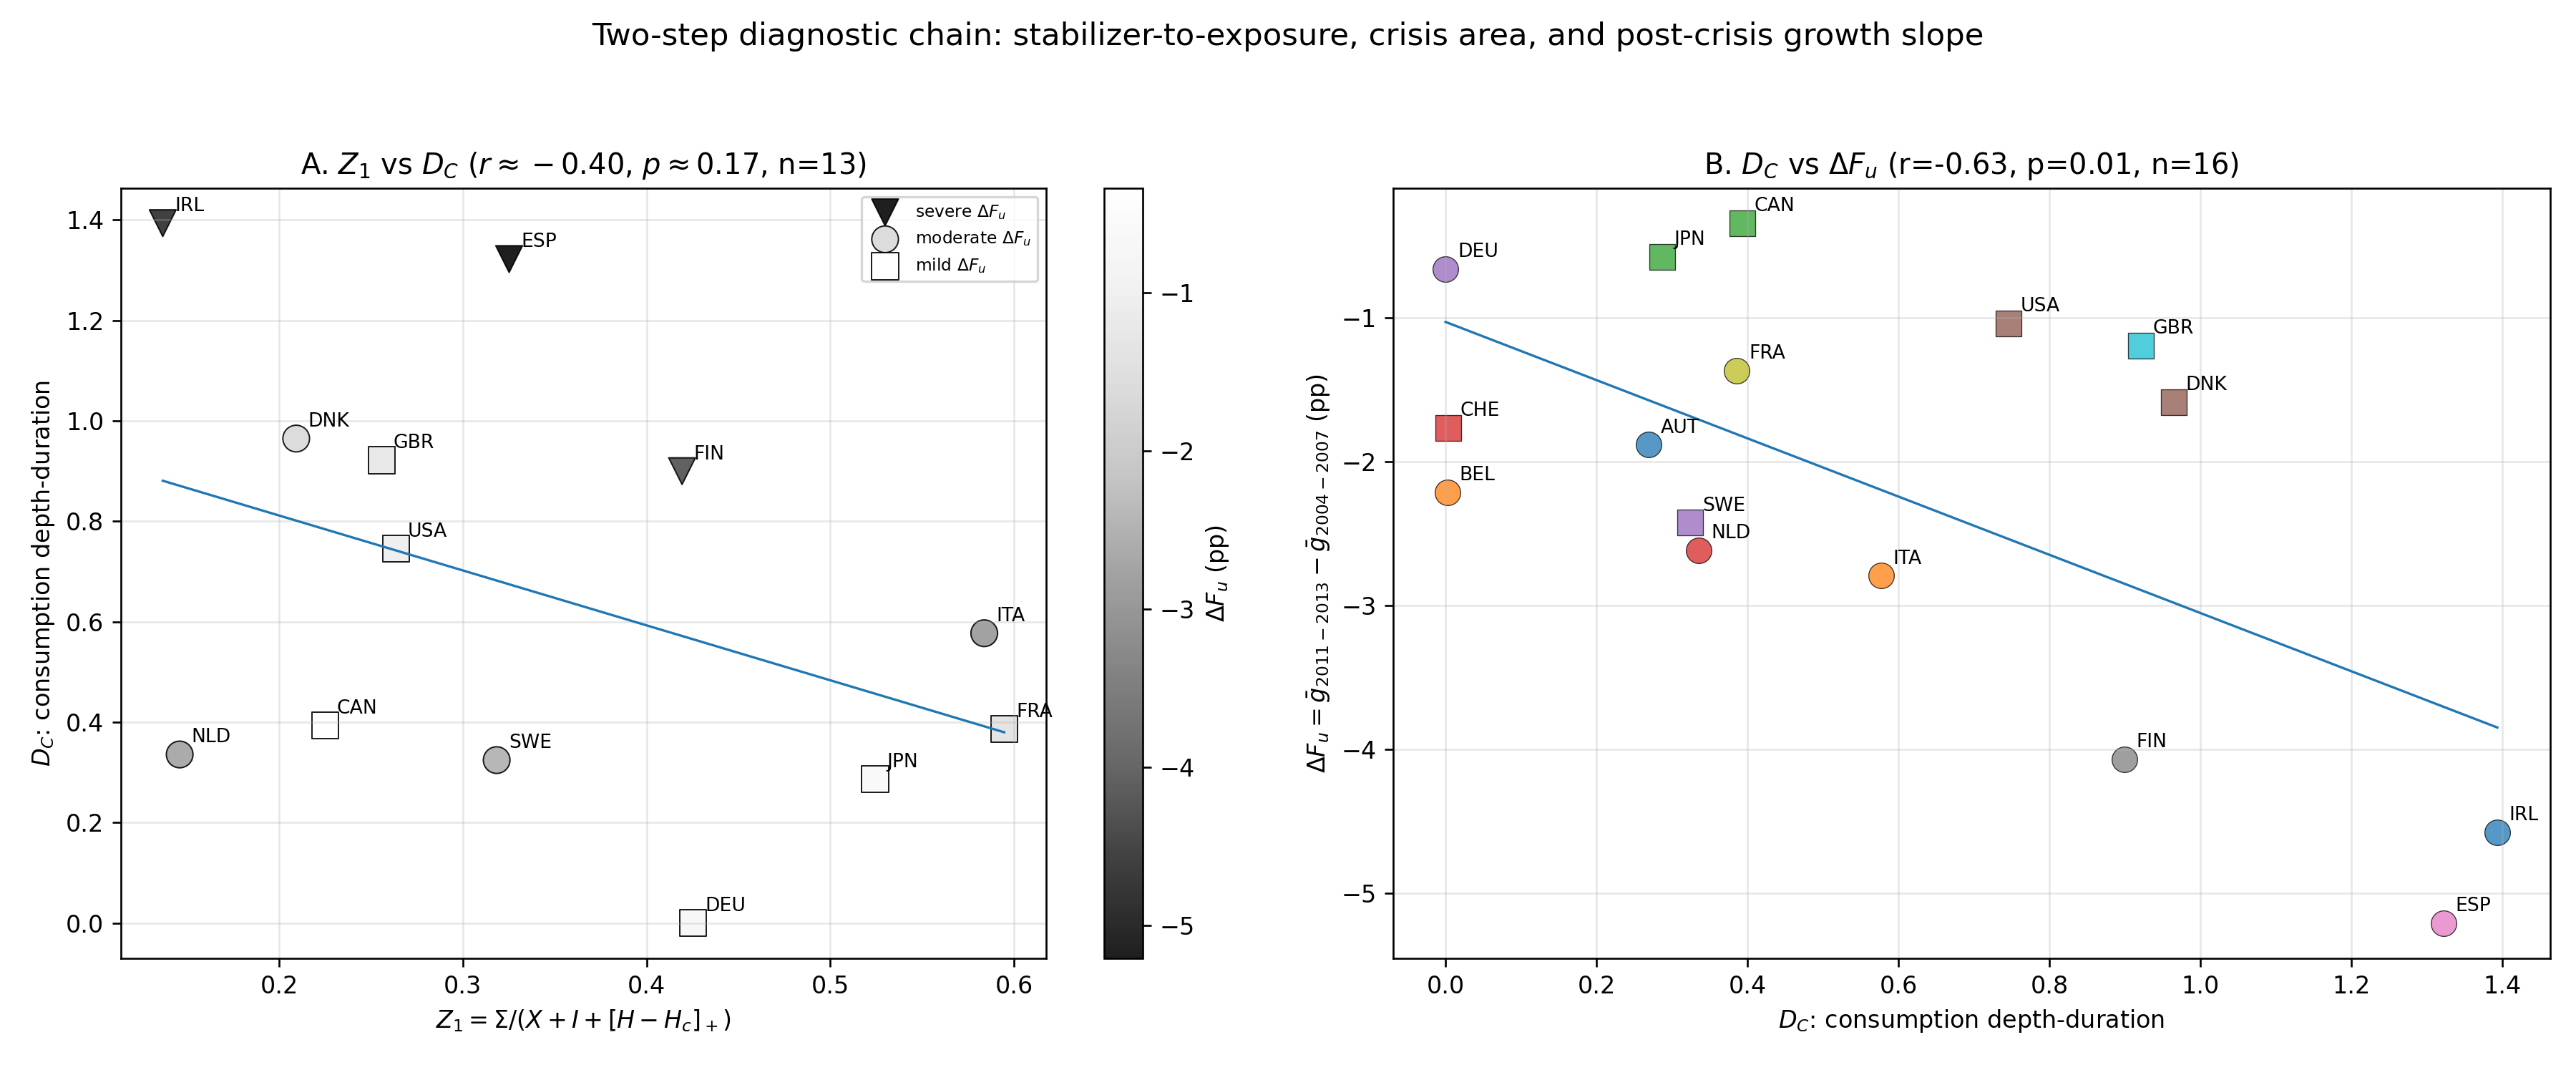
\includegraphics[width=0.98\textwidth]{figures/fig8_Z1_DC_DeltaFu_chain.png}
\caption{Two-step empirical diagnostic suggested by the normal form. Left: crisis depth-duration $D_C$ versus the stabilizer-to-exposure proxy $Z_1$ in the core sample. Point shading and marker shape indicate deterioration in post-rebound growth slope $\Delta F_u$ so that the panel remains interpretable in grayscale. Shapes encode $\Delta F_u$ bins: triangles, severe deterioration ($\Delta F_u<-3.0$ pp); circles, moderate deterioration ($-3.0\leq\Delta F_u<-1.5$ pp); squares, mild or weakest deterioration ($\Delta F_u\geq -1.5$ pp). The first link has the expected sign but is not significant at conventional levels, $r\approx -0.40$, $p\approx0.17$ for $n=13$. Right: $\Delta F_u$ versus $D_C$ in the extended WDI diagnostic sample. The second link is the strongest empirical diagnostic in the present pilot: $r=-0.63$ for $n=16$, with a 95\% Fisher interval approximately $[-0.86,-0.19]$. The figure supports a mediation-style reading, $Z_1\rightarrow D_C\rightarrow\Delta F_u$, but does not establish causal identification. Austria, Belgium, and Switzerland are included only in the WDI-based right panel in the present pilot.}
\label{fig:FuPhase}
\end{figure}

\begin{figure}[H]
\centering
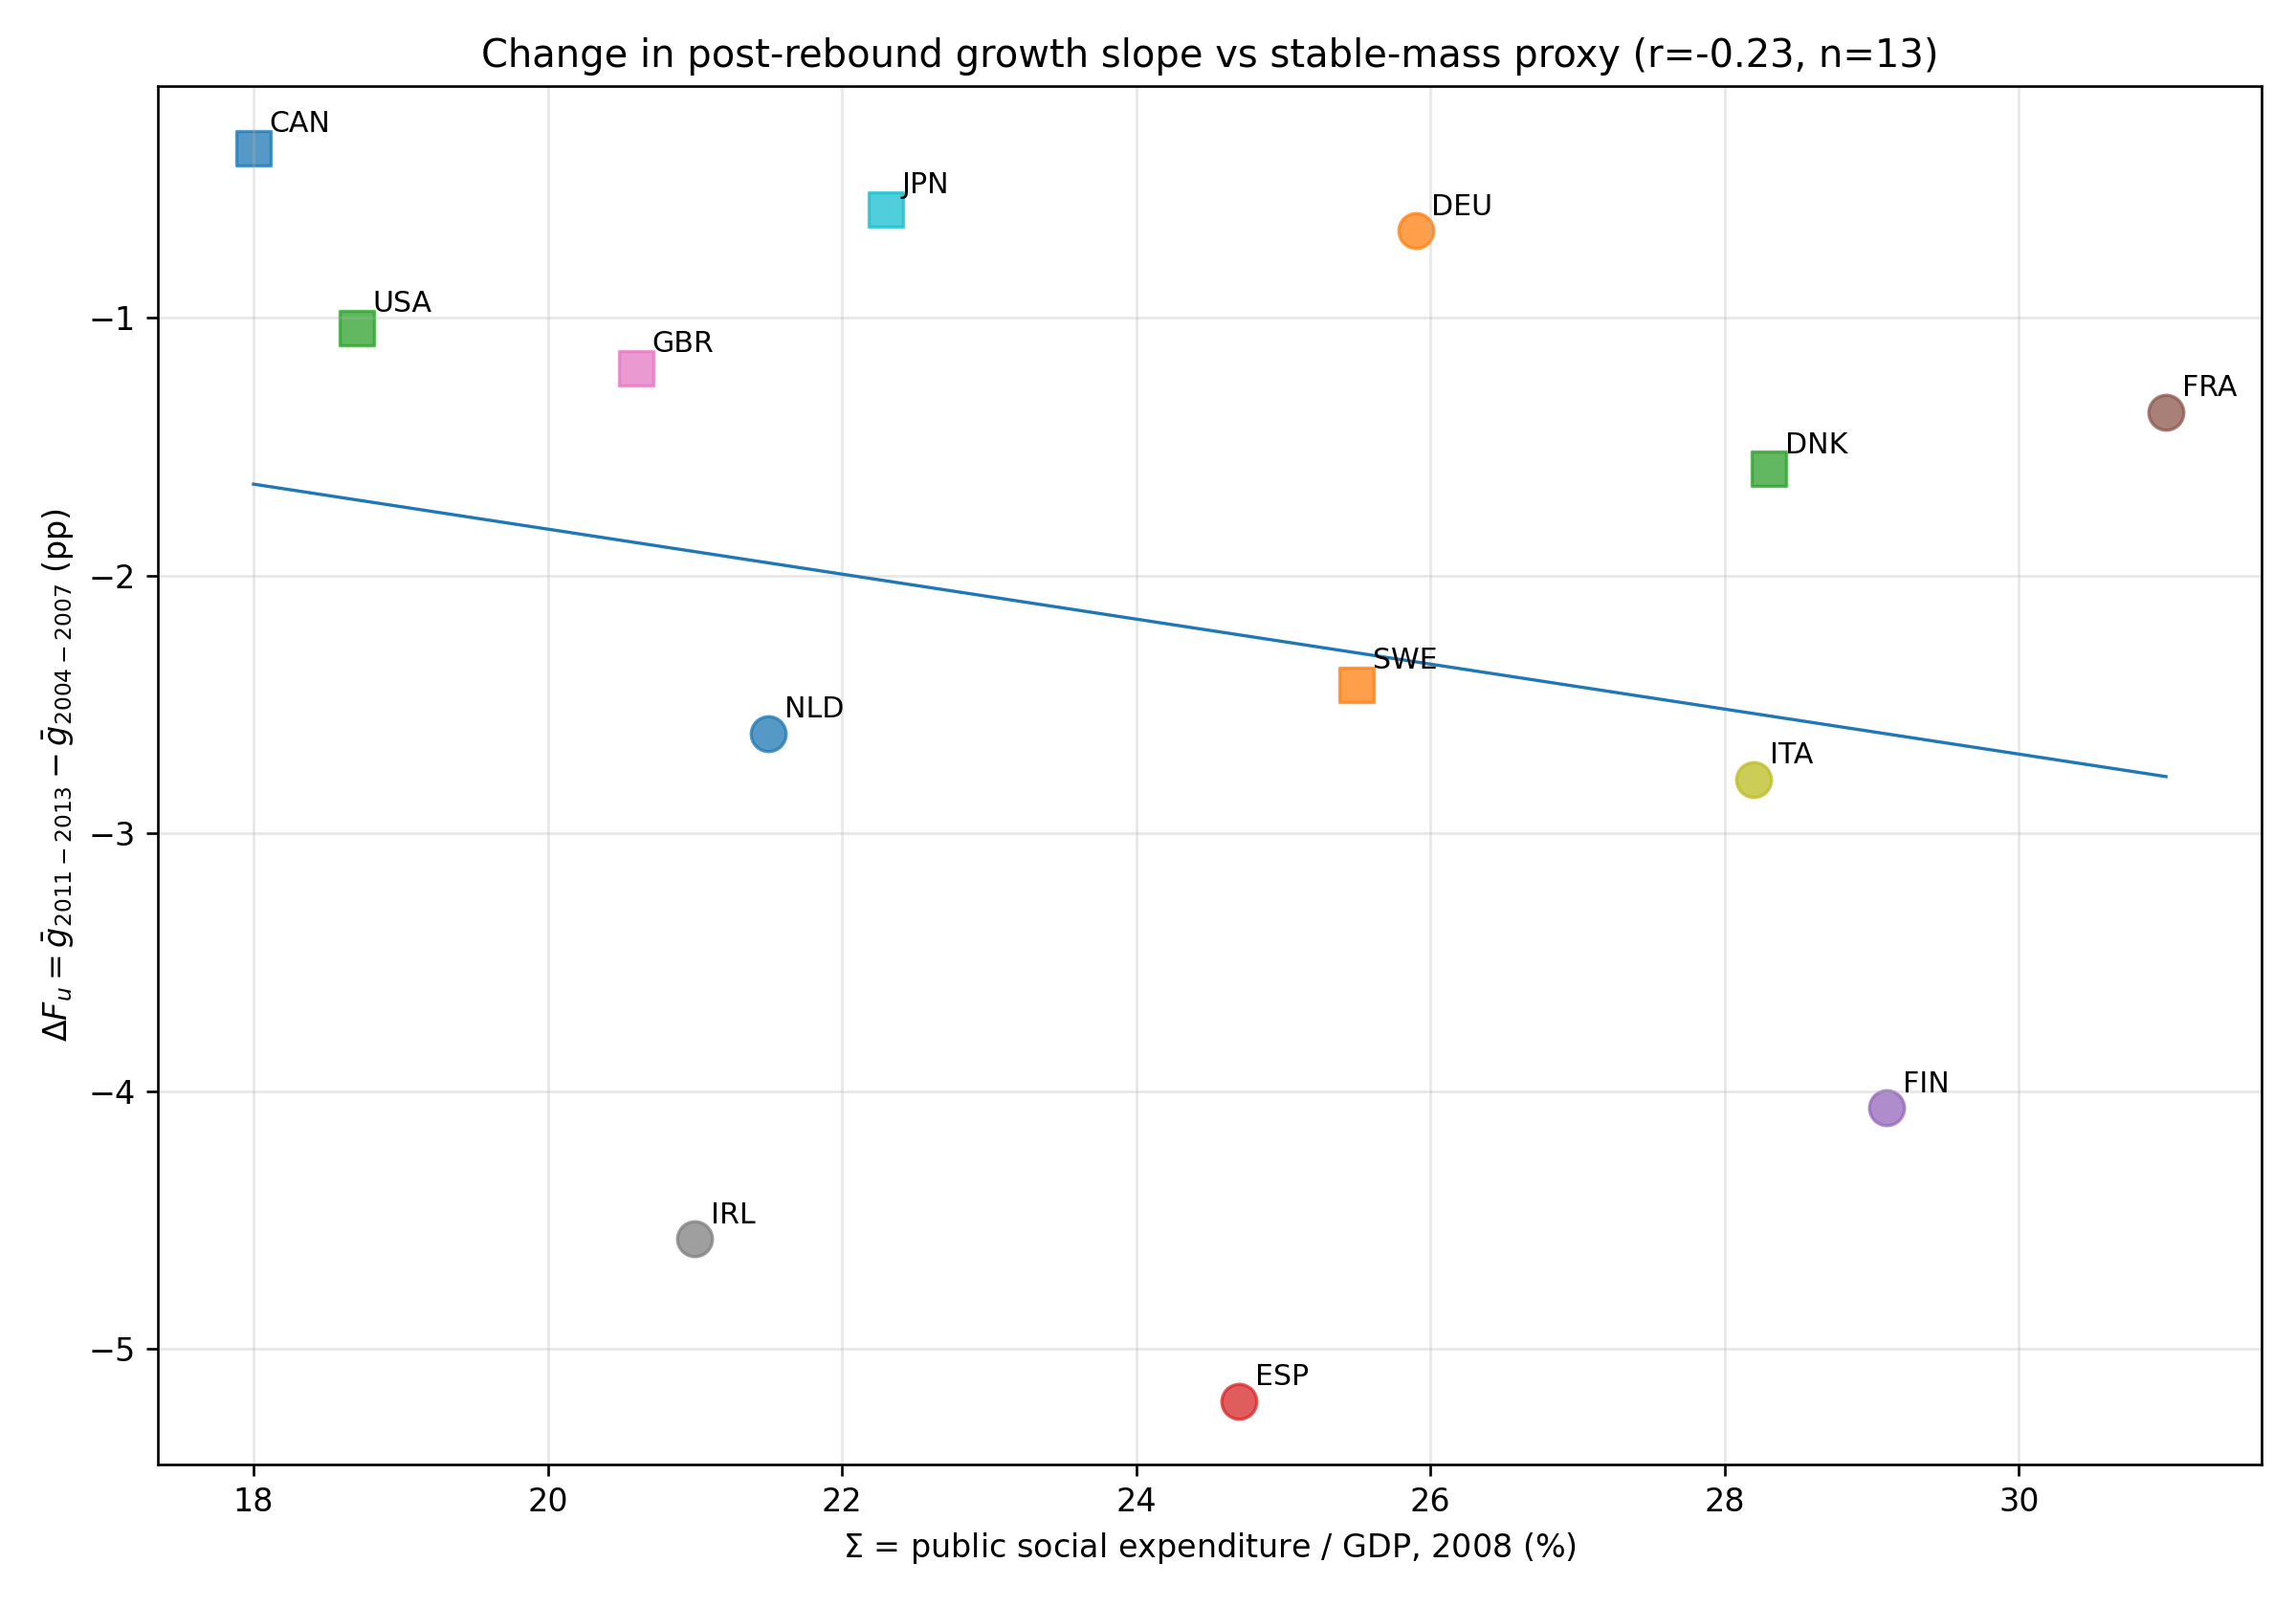
\includegraphics[width=0.95\textwidth]{figures/fig9_DeltaFu_vs_Sigma.png}
\caption{Change in post-rebound growth slope versus the narrow stable-mass proxy $\Sigma$. This panel tests the most indirect side of the model: the net relation between stable mass and post-crisis growth. The correlation is weak, $r=-0.23$, with a wide Fisher interval, approximately $[-0.69,0.37]$. This is consistent with the model's ambiguity: stable mass may reduce pure tangential acceleration, but by limiting threshold damage it may also preserve recovery capacity.}
\label{fig:DeltaFu}
\end{figure}

Figure~\ref{fig:DeltaFu} is therefore not expected to show a clean one-to-one relation. The $\Sigma\rightarrow\Delta F_u$ pathway combines two opposing effects: direct inertial resistance to tangential acceleration and indirect preservation of recovery capacity through reduced crisis depth-duration. The weak observed correlation supports the more cautious interpretation: the coupling pathway $D_C\rightarrow\Delta F_u$ is clearer in the pilot than the net growth-inertia relation $\Sigma\rightarrow\Delta F_u$.


\subsection{Household-debt threshold sensitivity}
\label{sec:HcSensitivity}
A possible concern is that the baseline household-debt threshold $H_c=60\%$ is tuned to the pilot sample. To test this, $Z_1$ was recomputed for three local threshold values, $H_c=50\%,60\%,70\%$, using the same core 13-country sample. The purpose of this check is not to estimate an optimal threshold, but to test whether the empirical sign pattern is stable under plausible local variation around the baseline value.

\begin{table}[H]
\centering
\caption{Sensitivity of the stabilizer-to-exposure coordinate to the household-debt threshold $H_c$. Pearson correlations, two-sided Pearson $p$-values, and Spearman correlations are reported for the core $Z_1$ scaling sample. The sign pattern is preserved across the tested thresholds: $Z_1$ remains positively associated with the shock-year relative-insulation coordinate $R_{2009}$ and negatively associated with the consumption depth-duration coordinate $D_C$. The $Z_1\to R_{2009}$ association is significant at conventional levels for the tested thresholds, whereas the upstream $Z_1\to D_C$ association is not.}
\label{tab:HcSensitivity}
\resizebox{\textwidth}{!}{%
\begin{tabular}{rrrrrrrr}
\toprule
$H_c$ & $r(Z_1,R_{2009})$ & $p_R$ & $\rho(Z_1,R_{2009})$ & $r(Z_1,D_C)$ & $p_D$ & $\rho(Z_1,D_C)$ & $n$ \\
\midrule
50\% & 0.564 & 0.045 & 0.593 & $-0.355$ & 0.233 & $-0.407$ & 13 \\
60\% & 0.612 & 0.026 & 0.604 & $-0.405$ & 0.170 & $-0.451$ & 13 \\
70\% & 0.584 & 0.036 & 0.604 & $-0.381$ & 0.199 & $-0.451$ & 13 \\
\bottomrule
\end{tabular}%
}
\end{table}

The threshold scan shows that the empirical signal is not driven by a knife-edge choice of $H_c$. The baseline value $H_c=60\%$ gives the strongest Pearson association within this local range, but the signs and magnitudes remain stable at $50\%$ and $70\%$. Spearman rank correlations show the same qualitative pattern. Leave-one-country-out checks likewise preserve the signs of the two associations for all three threshold values. Because this threshold scan is used as a local robustness check rather than as a search over independent hypotheses, the reported $p$-values are interpreted descriptively and no multiple-testing-adjusted discovery claim is made. The $60\%$ value is therefore used as a literature-anchored local marker for the onset of household balance-sheet stress, within a leverage-amplification literature in which household debt is nonlinear and state-dependent rather than harmful from the first unit of debt \cite{MianSufiVerner2017,KumhofRanciereWinant2015,JordaSchularickTaylor2013}. The baseline association is therefore not a knife-edge consequence of the precise $H_c=60\%$ placement.

The full sensitivity figures and leave-one-country-out table are provided in the reproducibility package under \texttt{figures/} and \texttt{data/}.

\section{Discussion}
\subsection{Role geometry, empirical scope, and directional stabilization}
The empirical results provide pilot evidence for a role geometry in a complex socioeconomic system. The core test is narrow: whether a scale-free stabilizer-to-fragility coordinate organizes the 2008--2009 OECD consumption response and shock-absorption diagnostics in a manner consistent with the proposed normal form. The article is therefore positioned as a reduced dynamical representation anchored by transparent country-level diagnostics.

The central object of the paper is the dynamical arrangement among stabilizing reservoir, thresholded fragility, and recovery motion. Crisis response and growth responsiveness are organized by shared roles: inertia, damping, forcing, restoring tendency, threshold activation, and coupled response geometry. Within this normal form, the same stable reservoir can act as protection in the transverse crisis mode and as inertia in the tangential growth mode.

The empirical layer anchors this role geometry in the 2008--2009 OECD episode. The $Z_1$ scaling, the country archetypes, and the growth-side diagnostics test whether the proposed control variables organize the response coherently. The strongest empirical diagnostics are the shock-absorption signal in the $Z_1$ scaling and the depth-duration coupling signal $D_C\to\Delta F_u$. The direct growth-inertia relation between $\Sigma$ and $\Delta F_u$ remains weak, making the growth side a target for larger-panel testing.

This framing turns stabilization into a directional problem. Productive recovery requires mobility along the tangential growth direction, whereas crisis prevention requires resistance to transverse displacement and to erosion of the effective distance from the crisis boundary. Stabilization is therefore not equivalent to maximal damping of all motion. The relevant objective is directional stabilization: protecting the boundary of the recovery basin while preserving motion along the recovery path. In this sense, the productive regime is not the absence of nonlinearity, but bounded nonlinear recovery motion protected from threshold-distance erosion.

The present nonlinear term produces threshold-amplified finite excursions. Full bifurcation analysis, damage memory, state-dependent restoring stiffness, or a second basin of attraction belong to a later dynamical-systems extension. Future economics-facing work should test the direct growth-inertia prediction with larger panels, multiple crisis windows, an explicit empirical mapping to $S_{\mathrm{crit}}$, and, if needed, a generalized model that separates $m_x(S)$ from $m_u(S)$.

\section{Conclusions}
The stabilizer-to-exposure ratio identifies a dimensionless empirical projection of the role-level control variable $Z_0$, and the oscillator model gives that projection a reduced dynamical interpretation. The central conceptual transition is
\[
\text{empirical projection}\quad\rightarrow\quad\text{dynamical role coordinate}.
\]
The ratio $Z_1$ is a narrow empirical shadow of $Z_0$: a role ratio between institutional reservoir and thresholded balance-sheet fragility. Stable inertial mass protects against transverse crisis displacement, but may reduce pure growth responsiveness. Household leverage matters because, above a coarse threshold, it begins to erode the distance to the crisis boundary. The resulting policy geometry is directional: stabilize the crisis boundary without suppressing recovery motion. In the current pilot, the shock-absorption and depth-duration coupling signals are more convincing than the direct growth-inertia signal; this asymmetry defines the next empirical task and motivates larger-panel tests across multiple crisis windows.


\section{Materials and methods}
\subsection{Reduced dynamical representation}
The following reduced dynamical representation defines the role geometry used in the Results section. It is specified as a minimal transparent model, not as a calibrated structural macroeconomic model.

\subsection{Dynamical roles, not physical identity}
The encounter between mechanics and economics is not an object-to-object identification. A socioeconomic system is not literally a mass on a spring, and the mechanical model is not decorative inspiration. The meeting point is mathematical: different systems may share dynamical roles.

The roles used here are inertia, damping, forcing, restoring tendency, threshold activation, and response geometry. This is the sense in which the analogy is used: not mechanical identity, but a reduced dynamical description in which different systems can share response roles. Throughout the paper, the phrase ``role-based normal form'' is used in this reduced-model sense, not in the strict bifurcation-theoretic sense of a canonical form obtained by near-identity transformations. The aim is to identify the minimal dynamical roles needed to describe crisis--recovery geometry in an interpretable way. The model asks whether crisis response can be described by a forced, damped, thresholded dynamical system in which the stabilizing component acts not only as damping but also as inertial mass.

\subsection{Relation to Goodwin--Keen dynamics}
The closest existing dynamical-economics lineage is the Goodwin--Keen family of models. Goodwin's growth-cycle model combined growth and cyclical dynamics in a stark nonlinear phase-space formulation \cite{Goodwin1967}. Empirical and econophysics-oriented work has also tested Goodwin growth-cycle dynamics in country-level data \cite{MouraRibeiro2013}. Keen extended this tradition in a Minsky-inspired direction by making private debt an endogenous instability variable \cite{Keen1995}. Subsequent work simplified and analyzed the Goodwin--Minsky--Keen structure \cite{Rammelt2019}, and recent control-theoretic work has represented the Keen model as an affine nonlinear system that can be modified through policy interventions \cite{PerezAvellaneda2024}.

The present model is not a replacement for that literature. It does not claim novelty in debt-driven nonlinear macroeconomic instability. The distinction is geometric. Unlike Goodwin--Keen models, which treat growth, cyclical fluctuation, employment, wage share, and private debt as coupled endogenous variables in a shared phase space, the present model imposes a decomposition between tangential growth momentum $u(t)$ and transverse crisis displacement $x(t)$. This decomposition is a modeling choice, not an empirical finding. Its purpose is to separate motion along a growth path from threshold-activated displacement away from that path.

In this sense, the proposed normal form is complementary to Goodwin--Keen dynamics. It gives priority to the geometry of response: one coordinate measures progress along a trajectory, while the other measures displacement from it. Household leverage enters as a thresholded transverse-fragility channel rather than as a fully endogenous debt-cycle state variable. The novelty claimed here is therefore narrower: the tangential/transverse decomposition, the stable-inertial-mass interpretation of stabilizing reservoirs, and the resulting trade-off frontier between crisis depth-duration and growth responsiveness.

\subsection{Two coordinates: growth and crisis}
We write an effective two-coordinate decomposition,
\begin{equation}
\bm{y}(t)=u(t)\bm{e}_u+x(t)\bm{e}_x,
\label{eq:state}
\end{equation}
where $\bm{e}_u$ and $\bm{e}_x$ denote idealized modeling directions rather than measured Euclidean axes. The decomposition is not a metric statement: it separates two roles, tangential motion along a development path and transverse displacement away from that path. We treat $u(t)$ and $x(t)$ as dynamically coupled but conceptually distinct coordinates. In the absence of explicit coupling terms, the two modes are taken not to drive each other directly; the coupling term introduced below explicitly allows transverse displacement to drag tangential motion.

This distinction matters. A crisis is not modeled merely as negative growth. It is a transverse activation: credit tightening, household deleveraging, unemployment-consumption feedback, liquidity stress, confidence loss, or consumption falling below trend. Micro evidence on consumption responses to unemployment is one motivation for treating consumption loss as a dynamic crisis channel rather than only a contemporaneous accounting outcome \cite{Fagereng2024}.

A concrete empirical realization of the crisis coordinate is
\begin{equation}
x(t)=\frac{C^{\mathrm{trend}}(t)-C(t)}{C^{\mathrm{trend}}(t)},
\label{eq:xdef}
\end{equation}
where $C(t)$ is real household consumption per capita and $C^{\mathrm{trend}}(t)$ is a pre-crisis trend. The corresponding depth-duration observable is
\begin{equation}
D_C=\int_{t_0}^{t_1}x_+(t)\,dt,
\qquad
x_+(t)=\brpos{x(t)}.
\label{eq:DC}
\end{equation}
The threshold-feedback term used below is different:
\begin{equation}
\brpos{x(t)-x_c}=\max(0,x(t)-x_c).
\label{eq:thresholdterm}
\end{equation}
This notation separates the positive crisis displacement $x_+(t)$ from displacement above the crisis threshold $x_c$.

For the growth coordinate, a simple representation is
\begin{equation}
u(t)=\log Y(t),
\end{equation}
where $Y(t)$ is real output per capita or a comparable real activity index. With this choice, $\dot u(t)=\dot Y(t)/Y(t)$ is the continuously compounded growth rate, and $\ddot u(t)$ is the time-rate of change of that growth rate. A constant percentage growth path is therefore represented as uniform tangential velocity.

\subsection{Stable inertial mass}
Let $S$ denote a stable socioeconomic reservoir: weakly cyclical income and expenditure streams that do not move one-for-one with the business cycle. In a narrow empirical proxy,
\[
S\sim \Sigma=\frac{\text{public social expenditure}}{GDP}.
\]
Theoretically, however, $S$ is broader. It may include social transfers, pensions, public wages, stable public demand, basic consumption, protected income streams, and other institutional flows. Defence expenditure, for example, is not part of the narrow SOCX social stabilizer, but persistent defence spending may contribute to stable inertial mass in countries where it forms a weakly cyclical institutional demand stream. Security shocks themselves would enter instead as transverse forcing. The narrow proxy $\Sigma$ is used because public social expenditure is consistently measured across the OECD pilot sample. The empirical pilot does not measure the full stable reservoir $S$; it tests whether a consistently measured component of $S$ already carries a detectable stabilizer-to-exposure signal. The broader $S$ is introduced to define the model's scope, not to make an empirical claim about defence spending, public wages, or other stable institutional flows in the present pilot.

The key modeling step is
\begin{equation}
m(S)=m_0+\alpha S,\qquad \alpha>0,
\label{eq:mS}
\end{equation}
\begin{equation}
c_x(S)=c_{x0}+\beta S,\qquad \beta>0.
\label{eq:cS}
\end{equation}
Thus $S$ contributes both to inertia and to damping. A stabilizer is not only a brake; it is stable inertial mass.

The use of the same $m(S)$ in the transverse and tangential equations below is a symmetry assumption of the minimal normal form. It expresses the idea that the same stable reservoir resists acceleration in both directions. The model does not require this equality in a calibrated setting: a generalized form with $m_x(S)=m_{x0}+\alpha_x S$ and $m_u(S)=m_{u0}+\alpha_u S$ would separate crisis inertia from growth inertia. The present paper uses the shared-mass case deliberately to expose the cleanest version of the trade-off.

\subsection{Crisis mode}
The transverse crisis mode is
\begin{equation}
m(S)\ddot{x}+c_x(S)\dot{x}+k_xx=F_x(t)+\kappa\brpos{x(t)-x_c}.
\label{eq:crisis}
\end{equation}
In Eq.~\eqref{eq:crisis}, $m(S)\ddot{x}$ represents inertial resistance to crisis acceleration, $c_x(S)\dot{x}$ damping of crisis displacement, $k_xx$ restoring tendency toward the pre-crisis path, $F_x(t)$ transverse crisis forcing, and $\kappa\brpos{x(t)-x_c}$ nonlinear crisis amplification after a threshold $x_c$ is crossed. Below threshold, the response remains an ordinary fluctuation. Above threshold, deleveraging, unemployment-consumption feedback, credit contraction, and confidence loss amplify the displacement.

Household leverage enters as a thresholded fragility channel. At the scaling level,
\begin{equation}
F_x\sim X+I+\brpos{H-H_c}.
\label{eq:Fx}
\end{equation}
This is the forcing representation of the same normal-form idea: leverage below $H_c$ contributes to ordinary exposure, while leverage above $H_c$ marks the beginning of threshold-distance erosion. An equivalent geometric representation is
\[
x_c(H)=x_{c0}-\gamma\brpos{H-H_c},
\]
where excess leverage contracts the crisis boundary rather than increasing the imposed shock. The minimal implementation uses the forcing representation and holds $x_c$ fixed, avoiding two simultaneous parameterizations of the same fragility channel. The essential point is geometric: a shock need not become larger for vulnerability to increase; it is enough for the effective distance to the nonlinear boundary to shrink.

This representation is related to macro-financial work in which credit allocation and debt overhang are state variables for vulnerability \cite{MullerVerner2024,Ivashina2024}, and to state-dependent fiscal-multiplier work in which the macroeconomic state, private debt, credit constraints, or financial-crisis regime changes the response to fiscal forcing \cite{Baum2012,BernardiniPeersman2018,BernardiniDeSchryderPeersman2020,McManus2020,FariaCastro2024}. Bernardini and Peersman find larger spending multipliers during private debt overhang \cite{BernardiniPeersman2018}, and Bernardini, De Schryder, and Peersman show that household indebtedness affects state-level government-spending multipliers around the Great Recession \cite{BernardiniDeSchryderPeersman2020}. In the notation used here, such state dependence is represented not by a multiplier alone, but by the system's position relative to a transverse crisis threshold.

\subsection{Growth mode}
The tangential growth mode is
\begin{equation}
m(S)\ddot{u}+c_u\dot{u}=F_u(t)-\lambda x_+(t).
\label{eq:growth}
\end{equation}
Here $F_u(t)$ is tangential growth forcing: innovation, investment, productivity, external demand, or other impulses that accelerate the economy along its growth path. The coupling term $-\lambda x_+(t)$ expresses that a transverse crisis displacement drags on growth momentum. The growth-mode damping coefficient is kept constant in the minimal toy model rather than written as $c_u(S)$. This is a conservative modeling choice: the empirical pilot directly motivates a stabilizer-dependent crisis damping channel, $c_x(S)$, but does not separately identify an additional stabilizer-dependent damping channel in pure growth motion. Stable reservoirs therefore enter the growth equation through shared inertia and through crisis drag, avoiding an extra free stabilizer-dependent parameter on the less identified growth side. The coupling is intentionally one-way in the minimal model: crisis displacement drags recovery, whereas recovery momentum is not allowed to feed back into the crisis boundary. This conservative closure avoids adding a fiscal-space, confidence, or endogenous-growth feedback channel that cannot be identified in the present pilot data.

Without this coupling, the model is only two independent oscillator-like equations. With it, the regimes become dynamically meaningful: low $S$ gives high growth responsiveness but threshold crossing; intermediate $S$ gives crisis protection without excessive inertia; high $S$ gives crisis protection but weaker pure tangential acceleration.

For short forcing intervals,
\[
\ddot{x}\sim \frac{F_x}{m(S)},\qquad \ddot{u}\sim \frac{F_u}{m(S)}.
\]
Therefore the same stable inertial mass suppresses crisis acceleration and limits growth acceleration. Stability is not simply beneficial and not simply costly. It is inertial.


\subsection{Empirical data sources and sample layers}
The empirical package uses processed reproducibility tables constructed from public aggregate databases. Public social expenditure as percent of GDP, $\Sigma$, is taken from the OECD Social Expenditure Database (SOCX). Household credit/debt as percent of GDP, $H$, is taken from the BIS total-credit statistics for the household sector. Exports of goods and services as percent of GDP, $X$, gross fixed capital formation as percent of GDP, $I$, GDP growth, household final consumption, and population are taken from the World Bank World Development Indicators. The processed tables are not raw database exports; they are reproducibility inputs sufficient to regenerate the manuscript figures and tables.

The core $Z_1$ scaling sample contains countries with complete stabilizer/exposure inputs, $\Sigma$, $X$, $I$, $H$, $Z_1$, the shock-year relative-insulation coordinate $R_{2009}$, the consumption depth-duration coordinate $D_C$, and growth-side diagnostics. The extended WDI diagnostic sample contains countries with WDI time-series quantities needed for $D_C$ and $\Delta F_u$ but incomplete stabilizer/exposure inputs in the current processed table. Extended-sample countries are used only for WDI-based diagnostics and are not used to support the $Z_1$ scaling claim.

\subsection{Construction of the depth-duration coordinate}
The time-axis recovery variables were generated by the WDI-processing script included in the reproducibility package. The script downloads WDI real-level series for 2000--2015: real GDP levels (\texttt{NY.GDP.MKTP.KN}), real household and NPISH final consumption expenditure (\texttt{NE.CON.PRVT.KN}), and population (\texttt{SP.POP.TOTL}). GDP and household consumption are divided by population to obtain real per-capita series, $Y_{pc,t}$ and $C_{pc,t}$.

For each country, a log-linear pre-crisis trend is fitted to real per-capita levels over 2000--2007 and extrapolated through 2015. The consumption depth-duration coordinate is then computed as the annual discrete sum of positive fractional shortfalls below the extrapolated trend over 2008--2015:
\begin{equation}
D_C=\sum_{t=2008}^{2015}
\left[\frac{C^{\mathrm{trend}}_{pc,t}-C_{pc,t}}{C^{\mathrm{trend}}_{pc,t}}\right]_+ .
\label{eq:DCmethods}
\end{equation}
The analogous GDP depth-duration coordinate $D_Y$ is computed by replacing $C_{pc,t}$ with $Y_{pc,t}$. Recovery-time diagnostics record the first post-2007 year in which the relevant per-capita series returns to its 2007 level, and the first post-2007 year in which the raw fractional gap to trend becomes non-positive. This construction makes $D_C$ the empirical discrete analogue of the model quantity $\int x_+(t)dt$.

\subsection{Empirical coordinates and statistical summaries}
The baseline stabilizer-to-exposure coordinate is computed as
\begin{equation}
Z_1=\frac{\Sigma}{X+I+[H-H_c]_+}, \qquad H_c=60\% .
\end{equation}
Threshold sensitivity recomputes the same coordinate for $H_c=50\%,60\%,70\%$ without refitting any additional parameters. The shock-year relative-insulation coordinate is
\begin{equation}
R_{2009}=g^{real}_{C,2009}-g^{real}_{Y,2009},
\end{equation}
where $g_C$ and $g_Y$ denote real household-consumption and real GDP growth. The post-rebound growth-slope diagnostic is
\begin{equation}
\Delta F_u=\overline{g}_{Y,2011-2013}-\overline{g}_{Y,2004-2007} .
\end{equation}
The manuscript reports Pearson correlations, two-sided Pearson $p$-values, and Spearman rank correlations for the core sample. Because the sample is small and the threshold scan is a robustness check rather than a threshold-selection procedure, the correlations are interpreted as descriptive pilot diagnostics rather than causal estimates.

\subsection{Toy dynamical model and reproduction}
The toy oscillator is parameter-transparent and is not calibrated to country data. Its purpose is to show how the same stable reservoir can reduce transverse crisis displacement while slowing tangential acceleration in a two-coordinate reduced dynamical representation. The illustrative parameters are listed in Table~\ref{tab:toyparams} and in the Python scripts under \texttt{code/}. Running the scripts listed in \texttt{README.md} regenerates the toy trajectories, phase portrait, threshold-regime map, linear-response figure, empirical scaling figures, and growth-forcing diagnostics from the included equations and processed CSV files.

\section*{Data Availability Statement}
All processed data and author-generated code required to reproduce the figures and tables are publicly available at Zenodo, DOI: \href{https://doi.org/10.5281/zenodo.20686861}{10.5281/zenodo.20686861}. The development repository is available at \url{https://github.com/eliezerkeinan-ops/stabilizer-exposure-crisis-dynamics}. The raw source data are publicly available from the OECD Social Expenditure Database (SOCX), BIS total credit statistics, and the World Bank World Development Indicators, as documented in the repository.

\section*{Funding Statement}
The author received no specific funding for this work.

\section*{Competing Interests Statement}
The author declares no competing interests.

\section*{Ethics Statement}
This study uses only publicly available, country-level aggregate economic data and does not involve human participants, animal subjects, or identifiable private information.

\appendix
\section{Reproducibility note}
The package includes processed reproducibility datasets under \texttt{data/}, scripts under \texttt{code/}, figure files under \texttt{figures/}, and supplementary GIF animations. The empirical tables are processed reproducibility datasets, not raw database exports. Source databases, variable definitions, and transformations are documented in \texttt{data\_sources.md}. Running the Python scripts listed in \texttt{README.md} regenerates the toy-model figures, phase portrait, threshold map, and empirical diagnostic figures from the included CSV files. The first script documents the raw WDI processing used to construct the depth-duration variables. The animations are conceptual toy-model visualizations and are not fitted country simulations.

\begin{thebibliography}{99}
\bibitem{MantegnaStanley1999} R. N. Mantegna and H. E. Stanley, \emph{An Introduction to Econophysics: Correlations and Complexity in Finance}, Cambridge University Press, 1999.
\bibitem{LuxMarchesi1999} T. Lux and M. Marchesi, ``Scaling and criticality in a stochastic multi-agent model of a financial market,'' \emph{Nature}, 397, 498--500, 1999.
\bibitem{SornetteJohansen1997} D. Sornette and A. Johansen, ``Large financial crashes,'' \emph{Physica A: Statistical Mechanics and its Applications}, 245, 411--422, 1997.
\bibitem{SornetteOuillon2012} D. Sornette and G. Ouillon, ``Dragon-kings: Mechanisms, statistical methods and empirical evidence,'' \emph{European Physical Journal Special Topics}, 205, 1--26, 2012.

\bibitem{Scheffer2009} M. Scheffer, J. Bascompte, W. A. Brock, V. Brovkin, S. R. Carpenter, V. Dakos, H. Held, E. H. van Nes, M. Rietkerk, and G. Sugihara, ``Early-warning signals for critical transitions,'' \emph{Nature}, 461, 53--59, 2009.
\bibitem{HaldaneMay2011} A. G. Haldane and R. M. May, ``Systemic risk in banking ecosystems,'' \emph{Nature}, 469, 351--355, 2011.
\bibitem{Battiston2016} S. Battiston, J. D. Farmer, A. Flache, D. Garlaschelli, A. G. Haldane, H. Heesterbeek, C. Hommes, C. Jaeger, R. May, and M. Scheffer, ``Complexity theory and financial regulation,'' \emph{Science}, 351, 818--819, 2016.
\bibitem{GuckenheimerHolmes1983} J. Guckenheimer and P. Holmes, \emph{Nonlinear Oscillations, Dynamical Systems, and Bifurcations of Vector Fields}, Springer, 1983.
\bibitem{OECD_SOCX} OECD, \emph{Social Expenditure Database (SOCX): Social expenditure aggregates}. OECD Data Explorer. Dataset used for public social expenditure as percent of GDP. \url{https://www.oecd.org/en/data/datasets/social-expenditure-database-socx.html}
\bibitem{BIS_TC} Bank for International Settlements, \emph{Credit to the non-financial sector}. BIS total credit statistics. Dataset used for household credit-to-GDP. \url{https://data.bis.org/topics/TOTAL_CREDIT}
\bibitem{WorldBank_WDI} World Bank, \emph{World Development Indicators}. Series used for GDP growth, household final consumption expenditure, exports of goods and services as percent of GDP, gross fixed capital formation, and population. \url{https://databank.worldbank.org/source/world-development-indicators}
\bibitem{Goodwin1967} R. M. Goodwin, ``A growth cycle,'' in C. H. Feinstein (ed.), \emph{Socialism, Capitalism and Economic Growth}, Cambridge University Press, pp. 54--58, 1967.
\bibitem{MouraRibeiro2013} N. J. Moura and M. B. Ribeiro, ``Testing the Goodwin growth-cycle macroeconomic dynamics in Brazil,'' \emph{Physica A: Statistical Mechanics and its Applications}, 392(9), 2088--2103, 2013.
\bibitem{Keen1995} S. Keen, ``Finance and economic breakdown: Modeling Minsky's financial instability hypothesis,'' \emph{Journal of Post Keynesian Economics}, 17(4), 607--635, 1995.
\bibitem{Rammelt2019} C. F. Rammelt, ``The dynamics of financial instability: Simplifying Keen's Goodwin--Minsky model,'' \emph{System Dynamics Review}, 35(1), 140--159, 2019.
\bibitem{PerezAvellaneda2024} I. Perez Avellaneda, F. Rosales, and L. A. Duffaut Espinosa, ``Feedback dynamic control for exiting a debt-induced spiral in a deterministic Keen model,'' \emph{PLOS ONE}, 19(2), e0295859, 2024.
\bibitem{Dolls2012} M. Dolls, C. Fuest, and A. Peichl, ``Automatic stabilizers and economic crisis: US vs. Europe,'' \emph{Journal of Public Economics}, 96(3--4), 279--294, 2012.
\bibitem{AuerbachFeenberg2000} A. J. Auerbach and D. Feenberg, ``The significance of federal taxes as automatic stabilizers,'' \emph{Journal of Economic Perspectives}, 14(3), 37--56, 2000.
\bibitem{McKayReis2016} A. McKay and R. Reis, ``The role of automatic stabilizers in the U.S. business cycle,'' \emph{Econometrica}, 84(1), 141--194, 2016.
\bibitem{MianSufiVerner2017} A. Mian, A. Sufi, and E. Verner, ``Household debt and business cycles worldwide,'' \emph{Quarterly Journal of Economics}, 132(4), 1755--1817, 2017.
\bibitem{KumhofRanciereWinant2015} M. Kumhof, R. Ranci\`ere, and P. Winant, ``Inequality, leverage, and crises,'' \emph{American Economic Review}, 105(3), 1217--1245, 2015.
\bibitem{JordaSchularickTaylor2013} O. Jorda, M. Schularick, and A. M. Taylor, ``When credit bites back: Leverage, business cycles, and crises,'' \emph{Journal of Money, Credit and Banking}, 45(s2), 3--28, 2013.
\bibitem{MullerVerner2024} K. M\"uller and E. Verner, ``Credit allocation and macroeconomic fluctuations,'' \emph{Review of Economic Studies}, 91(6), 3645--3676, 2024.
\bibitem{Ivashina2024} V. Ivashina, S. Kalemli-Ozcan, L. Laeven, and K. M\"uller, ``Corporate debt, boom-bust cycles, and financial crises,'' NBER Working Paper No. 32225, 2024.
\bibitem{Fagereng2024} A. Fagereng, H. Onshuus, and K. N. Torstensen, ``The consumption expenditure response to unemployment: Evidence from Norwegian households,'' \emph{Journal of Monetary Economics}, 146, 103578, 2024.
\bibitem{Baum2012} A. Baum, M. Poplawski-Ribeiro, and A. Weber, ``Fiscal multipliers and the state of the economy,'' IMF Working Paper WP/12/286, 2012.
\bibitem{BernardiniPeersman2018} M. Bernardini and G. Peersman, ``Private debt overhang and the government spending multiplier: Evidence for the United States,'' \emph{Journal of Applied Econometrics}, 33(4), 485--508, 2018.
\bibitem{BernardiniDeSchryderPeersman2020} M. Bernardini, S. De Schryder, and G. Peersman, ``Heterogeneous government spending multipliers in the era surrounding the Great Recession,'' \emph{Review of Economics and Statistics}, 102(2), 304--322, 2020.
\bibitem{McManus2020} R. McManus, F. G. Ozkan, and D. Trzeciakiewicz, ``Why are fiscal multipliers asymmetric? The role of credit constraints,'' \emph{Economica}, 88(349), 32--69, 2020.
\bibitem{FariaCastro2024} M. Faria-e-Castro, ``Fiscal multipliers and financial crises,'' \emph{Review of Economics and Statistics}, 106(3), 728--747, 2024.
\end{thebibliography}

\end{document}
